% \documentclass[aspectratio=169]{beamer}
\documentclass{beamer}
% \documentclass[notes]{beamer}

\usetheme[progressbar=foot, block=fill]{metropolis}

\usepackage{graphicx}
% \usepackage{booktabs}
% \usepackage{algorithm}
% \usepackage{algpseudocode}
\usepackage{subcaption}
\usepackage{pifont}
\usepackage{multirow}
\usepackage{booktabs}
\usepackage{tabularx}
\usepackage{caption}
\usepackage{pgf-pie}
% \usepackage{tikz}
% \usepackage{upgreek}
\usepackage{appendixnumberbeamer}
\usepackage{subcaption}
\usepackage{cleveref}
\usepackage{amsmath}
\usepackage{amsfonts}
\usepackage{pgfplots}
% \usepackage{url}
\usepackage{xfrac}
\usepackage{appendixnumberbeamer}

% \usetikzlibrary{calc}
% \usetikzlibrary{3d}
\usetikzlibrary{spy,arrows,shapes, arrows, positioning}

% \usepackage{biblatex}
\usepackage[backend=biber,style=authoryear,natbib=true]{biblatex} % Use the bibtex backend with the authoryear citation style (which resembles APA)
\addbibresource{references.bib}

\newcolumntype{L}{>{\raggedright\arraybackslash}X}

\newcommand\headercell[1]{%
   \smash[b]{\begin{tabular}[t]{@{}c@{}} #1 \end{tabular}}}

\newcommand{\cmark}{\ding{51}}%
\newcommand{\xmark}{\ding{55}}%

\graphicspath{ {images/} }

\title{Corner Localization and Camera Calibration from Imaged Lattices}
% \subtitle{A Novel Approach to Camera Calibration}
\author{Andrii Stadnik \inst{1} \and James Pritts \inst{2}}
\institute{
  \inst{1} Faculty of Computer Science, Ukrainian Catholic University, Lviv,
  Ukraine \\
  \inst{2} Czech Institute of Informatics, Robotics and Cybernetics at Czech Technical University in Prague, Czech
}
\date{2023}

% \metroset{}

\begin{document}

\begin{frame}[plain]
	\titlegraphic{\hfill
\includegraphics[height=1cm]{UCU-Apps2022_.png}}
	\titlepage
\end{frame}

% \begin{frame}
% 	\frametitle{Structure of the presentation}
% 	\tableofcontents
% \end{frame}

\section{Introduction}\label{sec:introduction}

\begin{frame}
	\frametitle{Camera calibration}

	Camera calibration is a necessary step for mapping from the pixel position to
	the real-world 3D position.

	\begin{alertblock}{Note}
		Here, we will use the term \textit{camera calibration} to refer to the
		geometric camera calibration.
	\end{alertblock}

	\begin{figure}
		\centering
		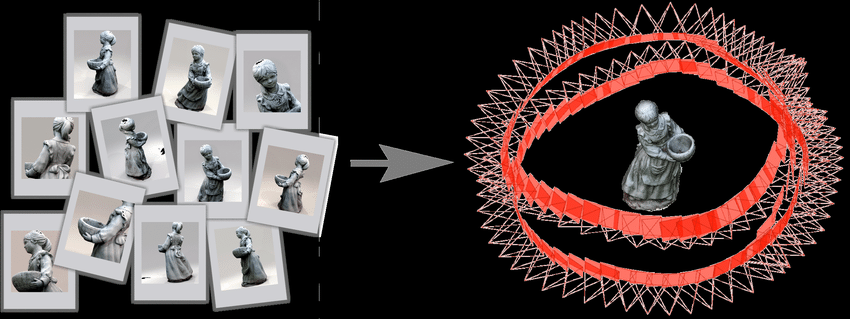
\includegraphics[width=0.8\textwidth]{3d_reconstruction.png}
		\caption{3D reconstruction}
	\end{figure}
\end{frame}

% \begin{frame}
% 	\frametitle{Motivation}
% 	Accurate camera calibration is required for many applications, such as:
% 	\begin{itemize}
% 		\item 3D reconstruction
% 		\item Robotics and automation
% 		\item Augmented reality
% 		\item Photogrammetry
% 		\item Stereo vision
% 	\end{itemize}
% \end{frame}

\begin{frame}
	\frametitle{Motivation}

	\begin{columns}[T,onlytextwidth]
		\column{0.6\textwidth}
		Accurate camera calibration is required for many applications, such as:
		\begin{itemize}
			\item 3D reconstruction
			\item Robotics and automation
			\item Augmented reality
			\item Photogrammetry
			\item Stereo vision
		\end{itemize}

		\column{0.4\textwidth}
		\begin{figure}
			\centering
			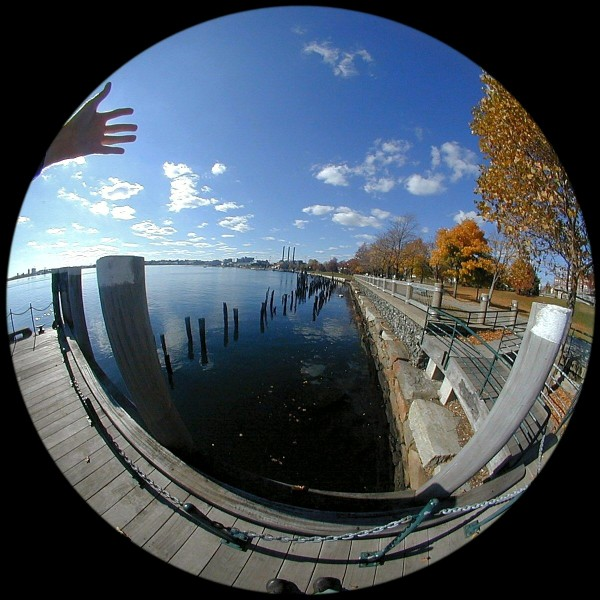
\includegraphics[width=0.8\textwidth]{high_distortion.png}
			\caption{Image with a high distortion}
		\end{figure}
	\end{columns}
\end{frame}

\begin{frame}
	\frametitle{Example}
	% \column{0.4\textwidth}
	\begin{figure}
		\begin{tikzpicture}[spy using outlines={circle,yellow,magnification=4,size=3cm, connect spies}]
			\node[anchor=south west,inner sep=0] (image) at (0,0)
			% {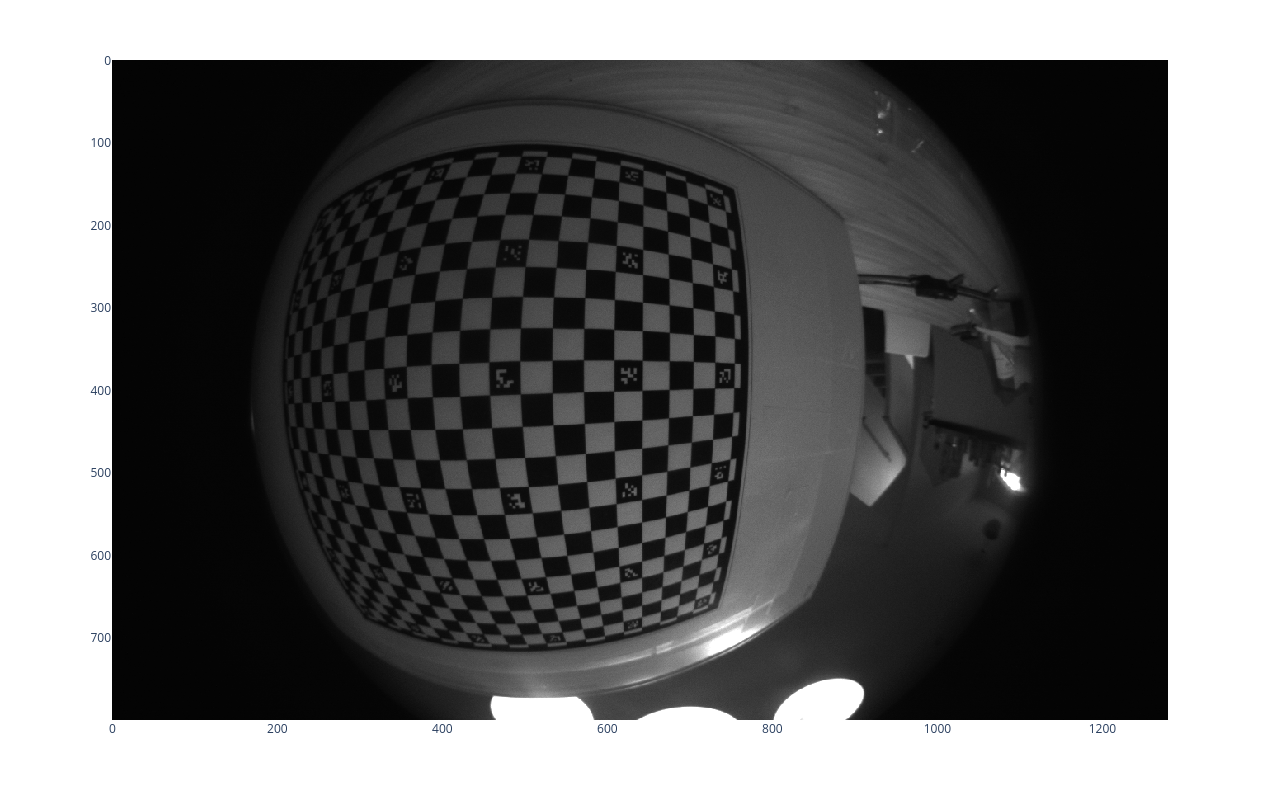
\includegraphics[width=0.6\textwidth]{distorted_image}};
			{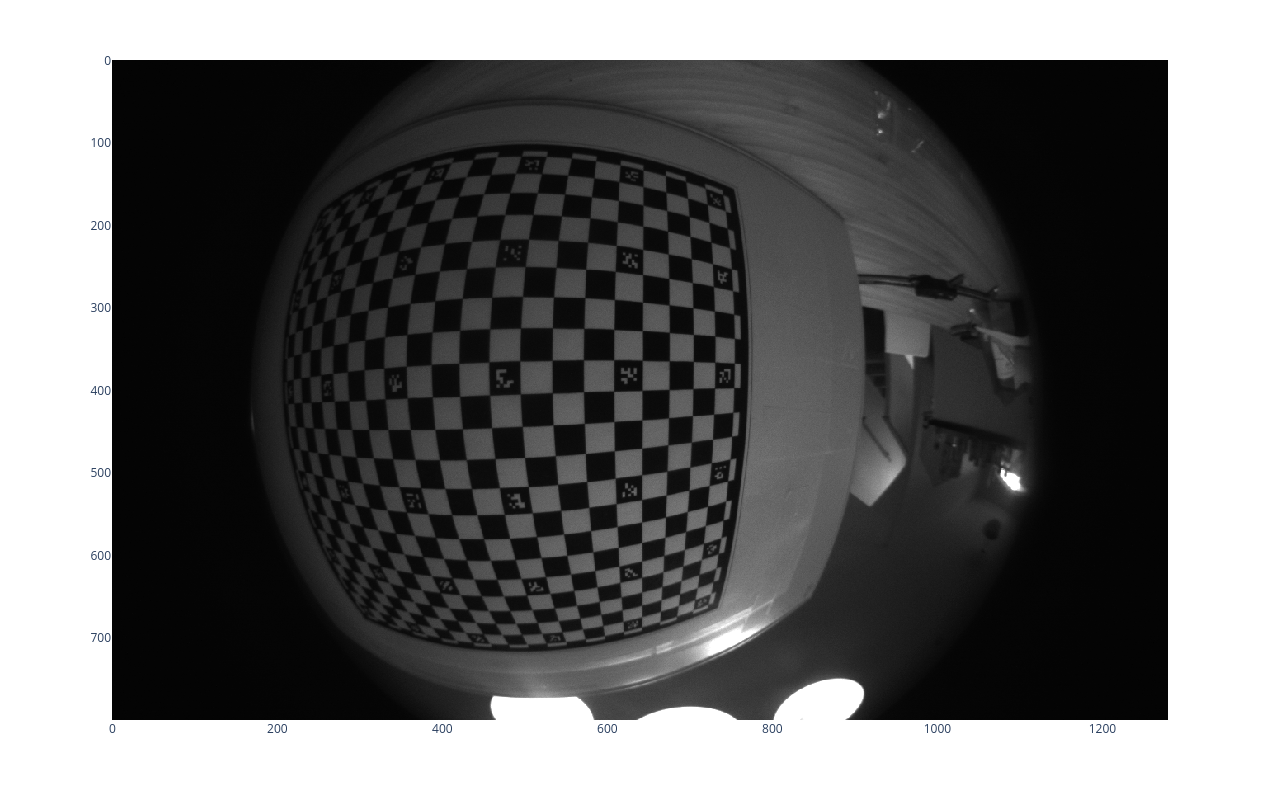
\includegraphics[width=0.8\textwidth]{distorted_image}};
			\begin{scope}[x={(image.south east)},y={(image.north west)}]
				\spy[red] on (2.5,1.4) in node [left] at (10.1,1.7);
				\spy[blue] on (3.5,3.0) in node [right] at (8.1,4.3);
			\end{scope}
		\end{tikzpicture}
		\caption{Corners near the center of the image and at the edge}
	\end{figure}
	% \end{columns}
\end{frame}

\begin{frame}
	\frametitle{Research objective}
	\textbf{Improve the detection of
		calibration board fiducials from calibration imagery taken by wide-angle or
		fisheye lenses.}

	% Add additional constrains to the camera
	% calibration by finding previously undetected features on the calibration
	% board.

	For that, we formulate the set of research questions:
	\begin{itemize}
		\item How to find additional features on the calibration board which were not
		      detected by the feature detector?
		\item How to filter out falsely detected features?
		\item Is there a need for finding additional features on the calibration
		      board? Are all of the points detected?
	\end{itemize}
\end{frame}

\section{Related work}\label{sec:related_work}

\begin{frame}
	\frametitle{TartanCalib\footcite{duisterhofTartanCalibIterativeWideAngle2022}}

	\begin{columns}
		\begin{column}{0.4\textwidth}
			\textbf{Algorithm}
			\begin{enumerate}
				\item Run the calibration toolchain
				\item Undistort the image
				\item Subpixel refinement
				\item Repeat
			\end{enumerate}
		\end{column}
		\begin{column}{0.6\textwidth}
			\textbf{Issues}
			\begin{itemize}
				\item Runs complete calibration toolchain each iteration
				\item Does not use the geometry information
				\item Not self-contained
			\end{itemize}
		\end{column}
	\end{columns}
\end{frame}

\begin{frame}
	\frametitle{Models comparison}
	\begingroup
	\scriptsize

	% \begin{figure}
	% 	\begin{subfigure}{0.45\linewidth}
	% 		\resizebox{\linewidth}{!}{
	% 			\centering
	% 			\begin{tikzpicture}
	% 				\begin{axis}[
	% 						xlabel={$x$},
	% 						ylabel={$y$},
	% 						grid=major,
	% 						title={Original board},
	% 					]
	% 					\addplot[
	% 						only marks,
	% 					] table {data/original_board.txt};
	% 				\end{axis}
	% 			\end{tikzpicture}
	% 		}
	\setlength\tabcolsep{1.5pt} % default value: 6pt
	\begin{table}
		\begin{tabularx}{\textwidth}{@{} L *{5}{c} @{}}
			\toprule
			\multicolumn{1}{c}{\multirow{2}{*}{\centering\textbf{Supports}}}           &
			\multicolumn{5}{c@{}}{\textbf{Name}}                                                           \\
			\cmidrule(l){2-6}                                                          &
			\textbf{OpenCV\footcite{dudaAccurateDetectionLocalization2018}}            &
			\textbf{TartanKalib\footcite{duisterhofTartanCalibIterativeWideAngle2022}} &
			\textbf{Kalibr\footcite{mayeSelfsupervisedCalibrationRobotic2013}}         &
			\textbf{OCamCalib\footcite{scaramuzzaToolboxEasilyCalibrating2006}}        &
			\textbf{LIBCBDETECT\footcite{geigerAutomaticCameraRange2012}}                                  \\
			\midrule
			Unknown board shape                                                        & \xmark & \cmark &
			\cmark                                                                     & \cmark & \cmark   \\
			\hline
			Occlusion                                                                  & \xmark & \cmark &
			\cmark                                                                     & \cmark & \cmark   \\
			\hline
			Model-based extra features detection                                       & \xmark & \cmark &
			\xmark                                                                     & \xmark & \xmark   \\
			\hline
			Geometry-based extra features detection                                    & \xmark & \xmark &
			\xmark                                                                     & \xmark & \xmark   \\
			\bottomrule
		\end{tabularx}
		\caption{Comparison of feature detectors}
	\end{table}
	\endgroup
\end{frame}

\section{Approach}\label{sec:approach}

% \section*{Intuition}\label{sec:intuition}
%
\begin{frame}
	\frametitle{Intuition (image)}
	Can you guess where the missing corners could be?

	% \begin{figure}
	% 	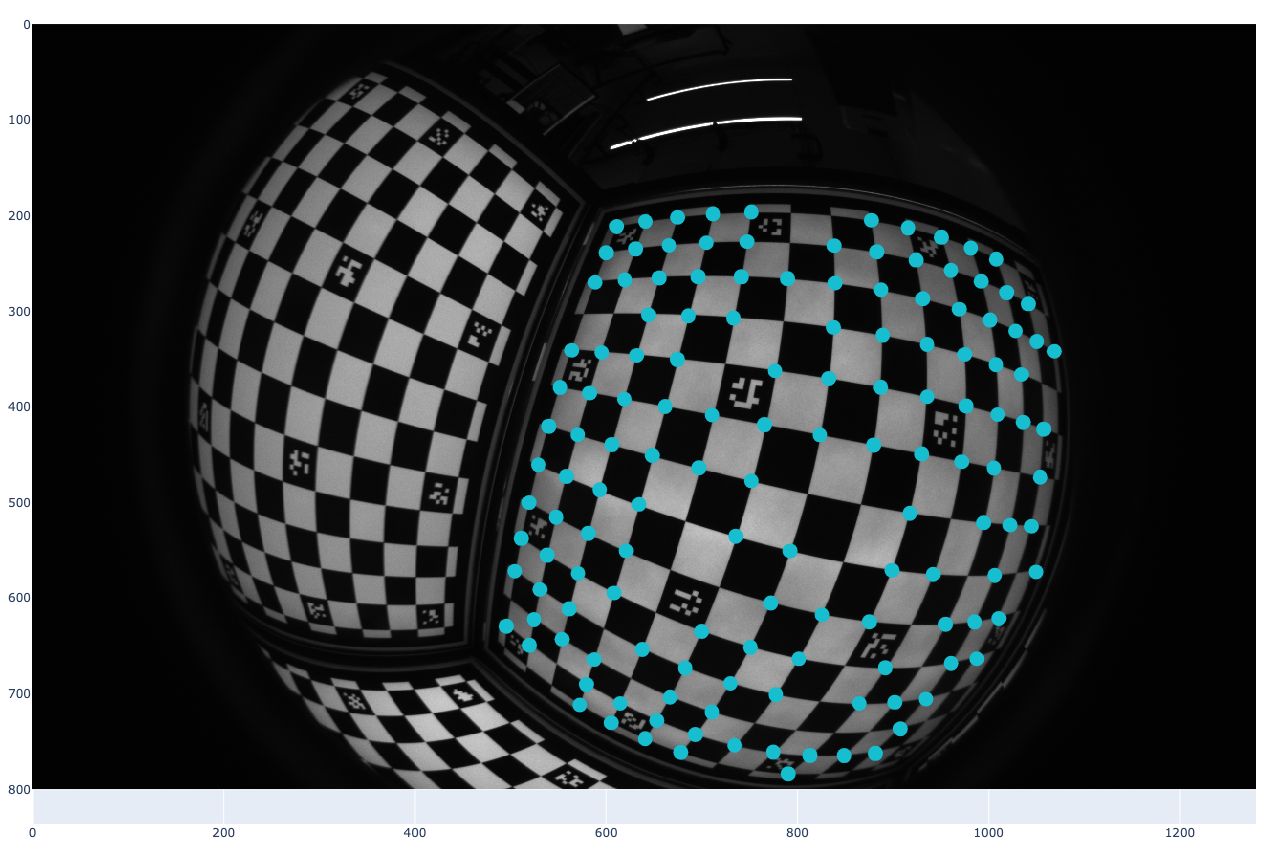
\includegraphics[width=0.7\textwidth]{example_board.png}
	% 	\caption{Example board detection}
	% \end{figure}
	\begin{figure}
		\begin{tikzpicture}[spy using outlines={circle,yellow,magnification=3,size=5cm, connect spies}]
			\node[anchor=south west,inner sep=0] (image) at (0,0)
			% {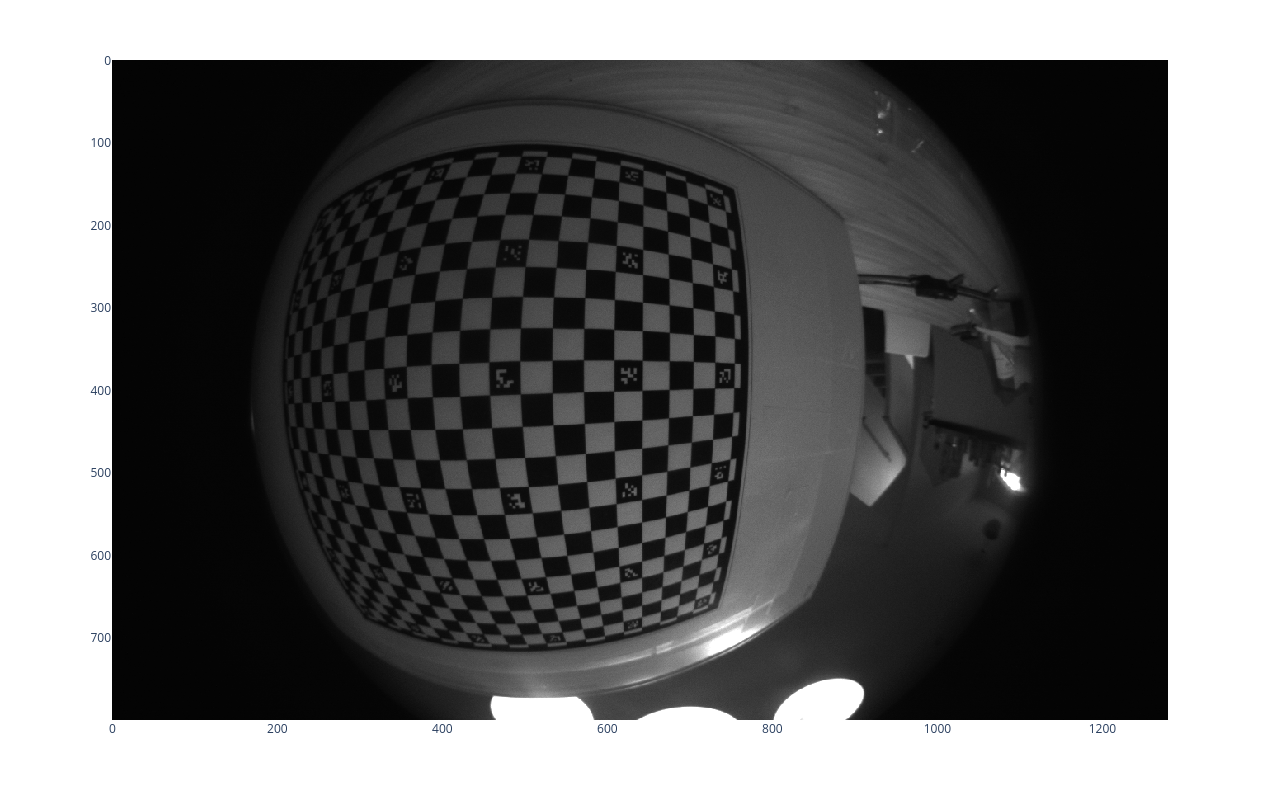
\includegraphics[width=0.6\textwidth]{distorted_image}};
			{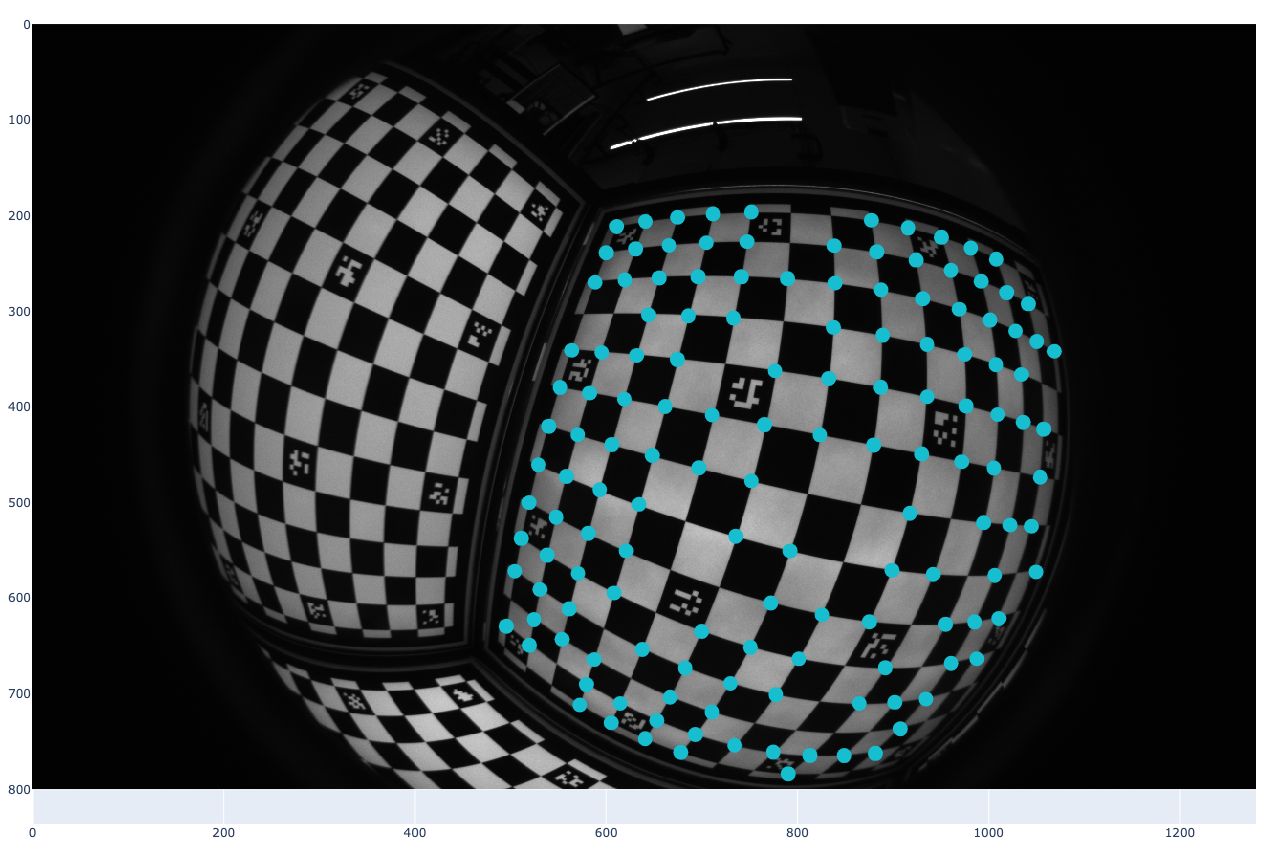
\includegraphics[width=0.7\linewidth]{example_board.png}};
			\begin{scope}[x={(image.south east)},y={(image.north west)}]
				% \spy[red] on (2.5,1.4) in node [left] at (10.1,1.7);
				\spy[blue] on (5.5,1.0) in node [right] at (6.5,3.3);
			\end{scope}
		\end{tikzpicture}
		\caption{Example board detection}
	\end{figure}
\end{frame}

\begin{frame}
	\frametitle{Intuition (corners)}
	Can you now?

	\begin{figure}
		\resizebox{0.7\textwidth}{!}{
			\centering
			\begin{tikzpicture}
				\begin{axis}[
						xlabel={$x$},
						ylabel={$y$},
						grid=major,
						title={Corners},
					]
					\addplot[
						only marks,
					] table {data/example_corners.txt};
				\end{axis}
			\end{tikzpicture}
		}
	\end{figure}
\end{frame}

\begin{frame}
	\frametitle{Intuition (board)}
	What about here?

	\begin{figure}
		\resizebox{0.7\textwidth}{!}{
			\centering
			\begin{tikzpicture}
				\begin{axis}[
						xlabel={$x$},
						ylabel={$y$},
						grid=major,
						title={Board},
					]
					\addplot[
						only marks,
					] table {data/example_board.txt};
				\end{axis}
			\end{tikzpicture}
		}
	\end{figure}
\end{frame}

\begin{frame}[standout]
	Use the board's geometry to find missing corners!
\end{frame}

\section*{Method}\label{sec:method}

\begin{frame}
	\frametitle{Pipeline overview}

	\begin{enumerate}
		\item Feature detection.
		\item Camera calibration.
		      \begin{enumerate}
			      \item Initialize camera parameters using the solver.
			      \item Refine camera parameters by optimization.
		      \end{enumerate}
		\item Impute the gaps in the board and extend it.
		\item Get positions of new points on the image.
		\item Filter out false positives.
	\end{enumerate}
\end{frame}

\begin{frame}
	\frametitle{Notation}
	The column vectors will be denoted by bold lowercase letters (e.g.
	\(\mathbf{u} = \begin{pmatrix}
		u, v, 1
	\end{pmatrix}^{T}\)), matrices will be denoted by uppercase letters (e.g.
	\(H = \begin{bmatrix}
		\mathbf{r_1} & \mathbf{r_2} & \mathbf{t}
	\end{bmatrix}
	\)). We will use homogeneous coordinates to simplify the equations.
\end{frame}

\begin{frame}
	\frametitle{Camera model}
	Camera parameters can be divided into 3 parts:
	\begin{itemize}
		\item Extrinsic parameters
		\item Distortion parameters
		\item Intrinsic parameters
	\end{itemize}

	They define a camera model, which
	projects a homogeneous 3D scene point
	\(\mathbf{x} = \begin{pmatrix}
		x, y, z, 1
	\end{pmatrix}^{T}\) into the homogeneous image point
	\(\mathbf{u} = \begin{pmatrix}
		u, v, 1
	\end{pmatrix}^{T}\).
\end{frame}

\begin{frame}
	\frametitle{Definition of the camera model}
	\begin{exampleblock}{Definition}
		\begin{align}
			\alpha \mathbf{u} & = K f_{\boldsymbol{\lambda}}(H\mathbf{x})
			\tag{Projection} \label{eq:projection}                                            \\
			\beta \mathbf{x}  & = H^{-1} g_{\boldsymbol{\lambda}}(K^{-1}\mathbf{u}) \tag{Back
				projection} \label{eq:back_projection}.
		\end{align}
		where \(K\) is the camera matrix, \(g_{\boldsymbol{\lambda}}(\cdot)\) is the division distortion
		model \footcite{fitzgibbonSimultaneousLinearEstimation2001}, \(f(\cdot)\) is the
		inverse of \(g(\cdot)\) and \(H\) is the homography matrix, and \(\alpha,
		\beta\) are non-zero scalars.
	\end{exampleblock}

	\begin{alertblock}{Note}
		You have printed materials with the details about the camera model.
		% Slides with the detailed explanation can be demonstrated upon request during the Q\&A session.
		% The explanation of the used camera model does not fit into the
		% presentation duration. However, the appendix of this presentation contains
		% the detailed explanation of each element of the equation, and will be
		% happily discussed/presented during the Q\&A session.
	\end{alertblock}

\end{frame}

\begin{frame}
	\frametitle{Feature detection}
	Use the approach, proposed by~\cite{geigerAutomaticCameraRange2012}:
	\begin{enumerate}
		\item Compute the corner likelihood map by convolving the image with two
		      \(n\times n\) prototypes.
		\item Additional filtering based on the number of the zero-crossings and
		      non-maximum suppression.
		\item Subpixel refinement of the detected corners.
		\item Board's structure refinement.
	\end{enumerate}
	\begin{figure}[h]
		\centering
		\begin{subfigure}{0.3\linewidth}
			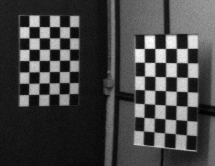
\includegraphics[width=\textwidth]{10.png}
			\caption{Input image}
		\end{subfigure}
		\begin{subfigure}{0.3\linewidth}
			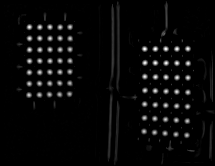
\includegraphics[width=\textwidth]{11.png}
			\caption{Corner likelihood}
		\end{subfigure}

		% \caption{Corner prototypes \citep{geigerAutomaticCameraRange2012}}
		\label{fig:corner_prototypes}
	\end{figure}

\end{frame}

\begin{frame}
	\frametitle{Camera calibration 1}

	Initialize camera parameters (\(R\), \(\mathbf{t}\),
	\(\boldsymbol{\lambda}\)) using the method, proposed by
	\cite{scaramuzzaToolboxEasilyCalibrating2006}.

	\begin{exampleblock}{Overview}
		The author proposes the multistage solver for the projection equation,
		assuming that the camera matrix is known.
	\end{exampleblock}
\end{frame}

\begin{frame}
	\frametitle{Camera calibration 2}

	Refine the values of \(R\), \(\mathbf{t}\), \(\boldsymbol{\lambda}\), and
	estimate \(K\) by minimizing the reprojection error between the
	board and the back-projected corners.

	\begin{exampleblock}{Reprojection error}
		The reprojection error is the distance between the reprojected point and the
		measured one:
		\begin{equation*}
			L = \sum_{i=1}^{N} \left\lVert
			H^{-1} g_{ \boldsymbol{\lambda}}(K^{-1} \mathbf{u_i}) -
			\mathbf{x_i} \right\rVert^2,
		\end{equation*}
		where \(\boldsymbol{\lambda}\) are the division distortion model
		parameters, \( \mathbf{x_{i}}\) and \(\mathbf{u_{i}}\) are the coordinates
		of the \(i\)-th corner in the 3D scene coordinates, and the respective
		feature on the image.
	\end{exampleblock}
\end{frame}

\begin{frame}
	\frametitle{Additional features detection}
	To find the probable positions of the previously undetected corners, we
	impute the gaps in the board, and extend it by 1 row and column from each
	side:
	\begin{figure}
		\begin{subfigure}{0.45\linewidth}
			\resizebox{\linewidth}{!}{
				\centering
				\begin{tikzpicture}
					\begin{axis}[
							xlabel={$x$},
							ylabel={$y$},
							grid=major,
							title={Original board},
						]
						\addplot[
							only marks,
						] table {data/original_board.txt};
					\end{axis}
				\end{tikzpicture}
			}
		\end{subfigure}
		\begin{subfigure}{0.45\linewidth}
			\resizebox{\linewidth}{!}{
				\centering
				\begin{tikzpicture}
					\begin{axis}[
							xlabel={$x$},
							ylabel={$y$},
							grid=major,
							title={Extended board},
						]
						\addplot[
							only marks,
						] table {data/extended_board.txt};
					\end{axis}
				\end{tikzpicture}
			}
		\end{subfigure}
	\end{figure}
\end{frame}

\begin{frame}
	\frametitle{Binary classification}
	\begin{itemize}
		\item Compute the corner likelihood map for the image.
		\item Use the ROC curve and pick the threshold which maximizes the G-mean.
	\end{itemize}

	We tested the approach of \cite{geigerAutomaticCameraRange2012}, and,
	alternatively, the Hessian responses for the image, as proposed by
	\cite{chenNewSubPixelDetector2005}.
\end{frame}

\section{Experiments}\label{sec:experiments}

\begin{frame}
	\frametitle{Metrics}
	The paper's main contribution is finding additional calibration boards' features, which
	then can be used as an input to any other camera calibration algorithm.

	\begin{itemize}
		\item Number of recovered artificially removed points
		\item Number of recovered points under occlusion
		\item Number of recovered points on original images
	\end{itemize}

\end{frame}

\begin{frame}
	\frametitle{Dataset}
	\textbf{OV} \citep{lochmanBabelCalibUniversalApproach2021} is a dataset of
	approximately 1400 images. It was collected using eight stereo cameras.
	As a calibration pattern, the checkerboard pattern with \(9\times 6\) tags of 22 mm size
	was used.

	\begin{alertblock}{Note}
		Much more data was collected. However, the initial feature detection
		supports only checkerboard patterns for now. Other than that, the pipeline
		works with any pattern.
	\end{alertblock}
\end{frame}

\begin{frame}
	\frametitle{Camera calibration 1}
	Compare the initial camera calibration with the camera calibration obtained via
	optimization of reprojection error.

	\begin{figure}
		\begin{subfigure}{0.45\linewidth}
			\resizebox{\linewidth}{!}{
				\begin{tikzpicture}
					\pie[rotate=90, explode=0.1, sum=auto, color={green!60, blue!60, red!60}, text=legend]{
						254/Correctly detected,
						80/Reprojection error > 10,
						458/Not correctly detected
					}
				\end{tikzpicture}
			}
			\caption{Initial calibration}
		\end{subfigure}
		\hfill
		\begin{subfigure}{0.45\linewidth}
			\resizebox{\linewidth}{!}{
				\begin{tikzpicture}
					\pie[rotate=90, explode=0.1, sum=auto, color={green!60, blue!60, red!60}, text=legend]{
						658/Correctly detected,
						19/Reprojection error > 10,
						115/Not correctly detected
					}
				\end{tikzpicture}
			}
			\caption{Final calibration}
		\end{subfigure}
	\end{figure}
\end{frame}

\begin{frame}
	\frametitle{Camera calibration 2}

	\begin{figure}
		% \begin{subfigure}{0.45\linewidth}
		\begin{subfigure}{\linewidth}
			\resizebox{\linewidth}{!}{
				\begin{tikzpicture}
					\begin{axis}[
							ybar interval,
							ymin=0,
							ylabel={Frequency},
							xlabel={Value},
							height=0.3\linewidth,
							width=\linewidth,
							ticklabel style = {font=\tiny},
							% title={Initial calibration}
						]
						\addplot+ [hist={data min=0,data max=10,bins=20}] table [y index=0]
							% \addplot+ [hist={bins=30}] table [y index=0]
							{data/reprojection_error_init.txt};
					\end{axis}
				\end{tikzpicture}
			}
			\caption{Initial calibration's reprojection error histogram}
		\end{subfigure}
		\begin{subfigure}{\linewidth}
			\resizebox{\linewidth}{!}{
				\begin{tikzpicture}
					\begin{axis}[
							ybar interval,
							ymin=0,
							ylabel={Frequency},
							xlabel={Value},
							height=0.3\linewidth,
							width=\linewidth,
							ticklabel style = {font=\tiny},
							% title={Reprojection error}
						]
						\addplot+ [hist={data min=0,data max=10,bins=20}] table [y index=0]
							% \addplot+ [hist={bins=30}] table [y index=0]
							{data/reprojection_error_final.txt};
					\end{axis}
				\end{tikzpicture}
			}
			\caption{Final calibration's reprojection error histogram (in px.)}
		\end{subfigure}
	\end{figure}

\end{frame}

\begin{frame}
	\frametitle{Additional features detection}

	\begin{columns}
		\begin{column}{0.6\textwidth}
			\begin{figure}
				\centering
				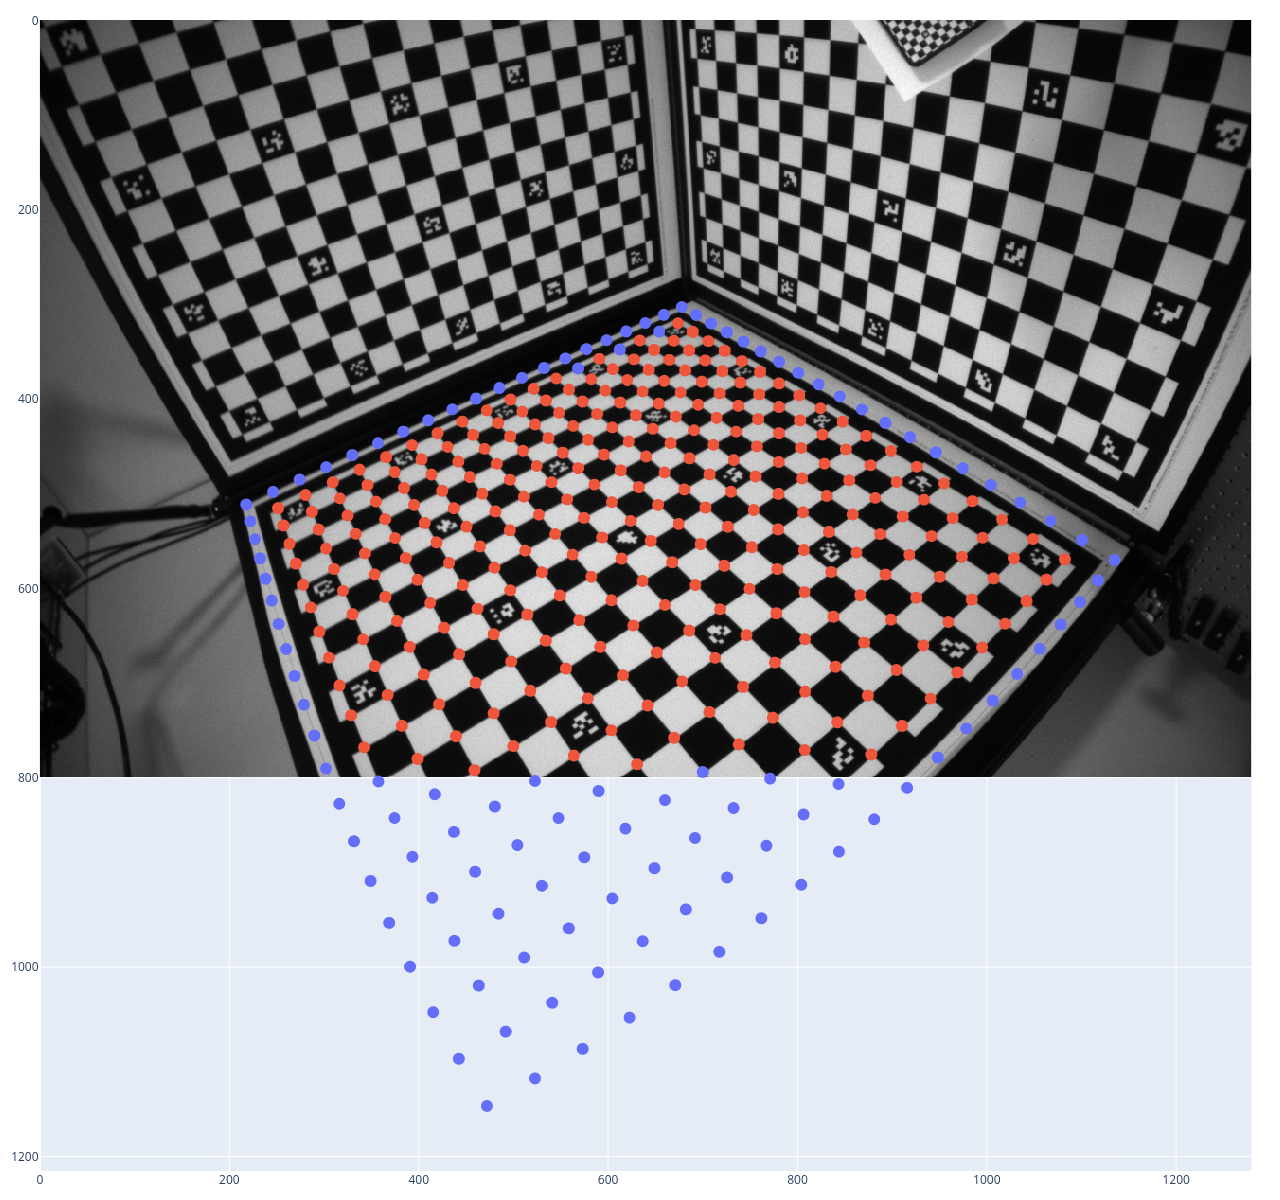
\includegraphics[width=\textwidth]{extended_board_img.png}
				\caption{Extended board, new points are marked as blue}
				\label{fig:extended_board_img}
			\end{figure}
		\end{column}
		\begin{column}{0.4\textwidth}
			\begin{figure}
				\begin{subfigure}{\textwidth}
					\resizebox{\textwidth}{!}{
						\begin{tikzpicture}
							\begin{axis}[
									xlabel={$x$},
									ylabel={$y$},
									grid=major,
									title={Original board},
								]
								\addplot[
									only marks,
								] table {data/original_board.txt};
							\end{axis}
						\end{tikzpicture}
					}
					% \caption{Original board}
				\end{subfigure}
				\begin{subfigure}{\textwidth}
					\resizebox{\textwidth}{!}{
						\begin{tikzpicture}
							\begin{axis}[
									xlabel={$x$},
									ylabel={$y$},
									grid=major,
									title={Extended board},
								]
								\addplot[
									only marks,
								] table {data/extended_board.txt};
							\end{axis}
						\end{tikzpicture}
					}
					% \caption{Extended board}
				\end{subfigure}
			\end{figure}
		\end{column}
	\end{columns}

\end{frame}

\begin{frame}
	\frametitle{Classification}

	The Hessian approach proved to be more robust, as the alternative gave too many false
	positives, especially for the edges.

	\begin{figure}
		\begin{subfigure}{0.30\linewidth}
			\begin{tikzpicture}[spy using outlines={circle,yellow,magnification=10,size=3cm, connect spies}]
				\node[anchor=south west,inner sep=0] (image) at (0,0)
				% {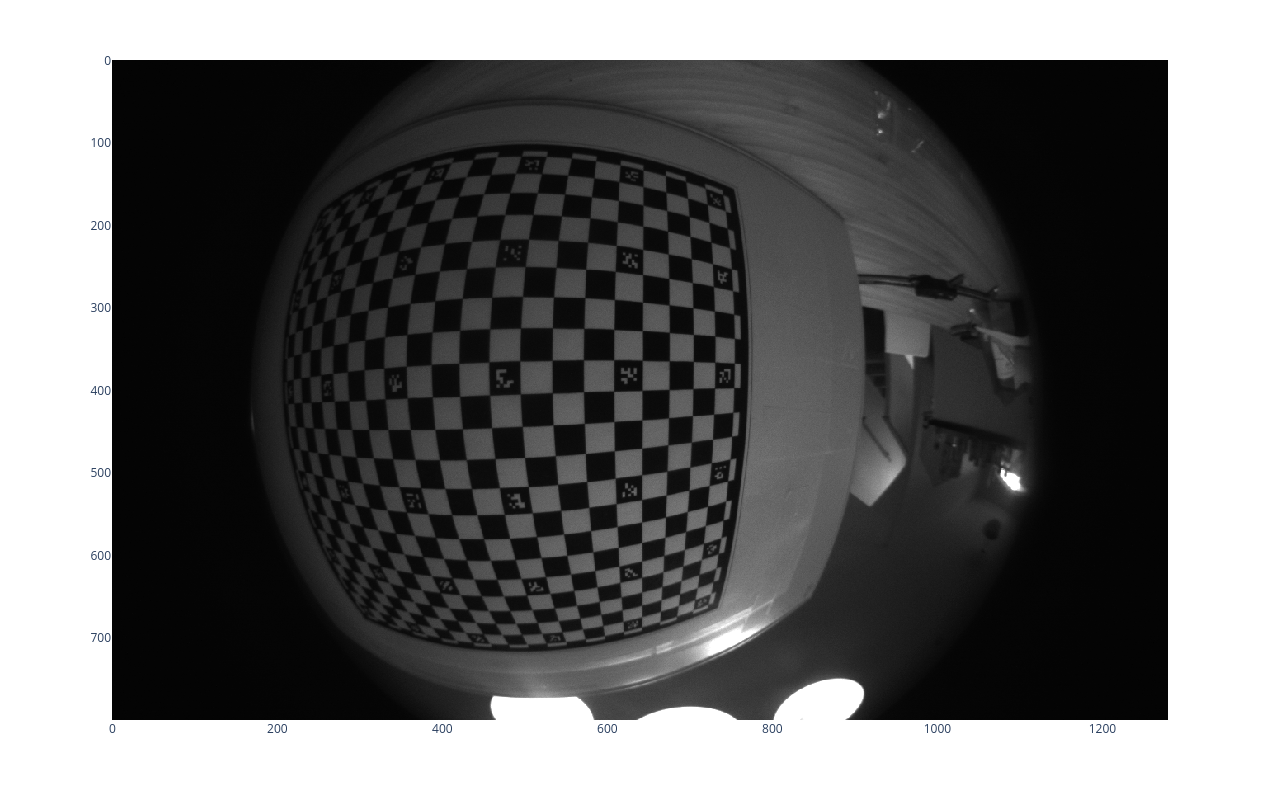
\includegraphics[width=0.10\textwidth]{distorted_image}};
				{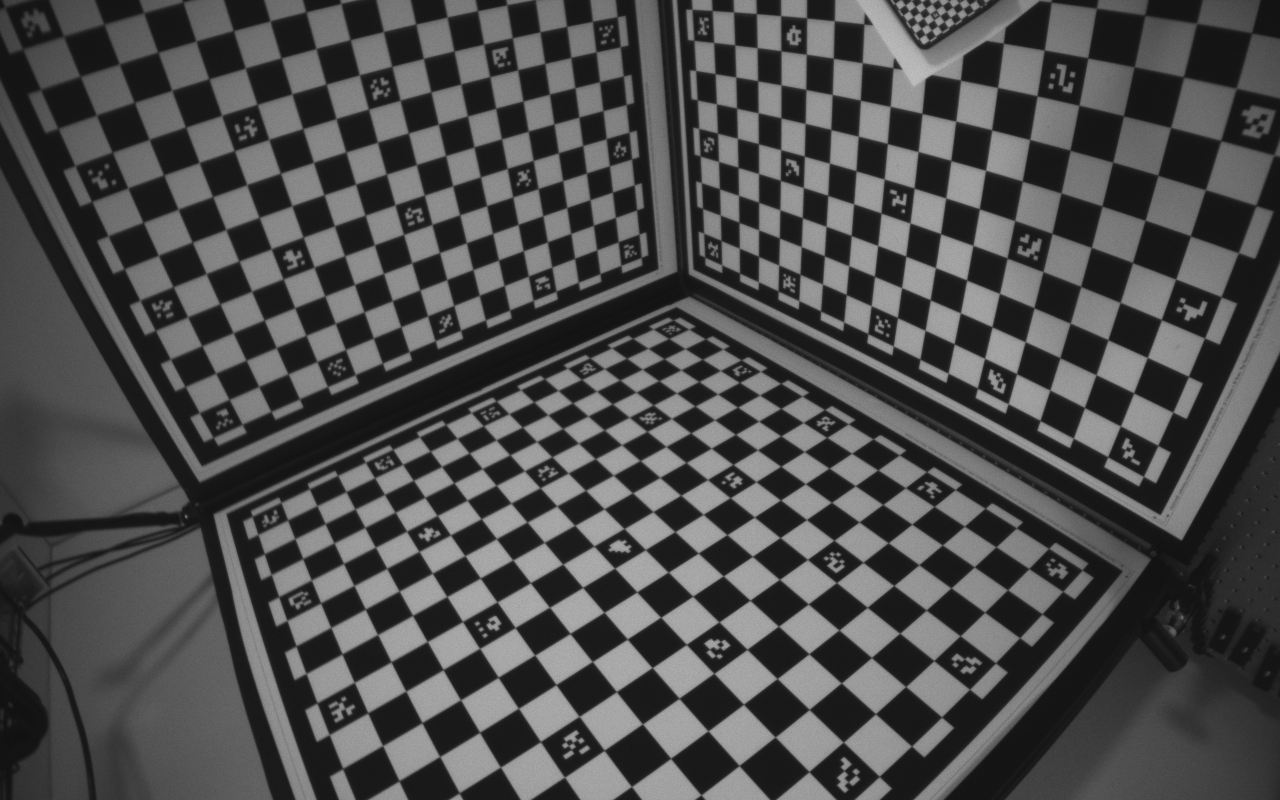
\includegraphics[width=\linewidth]{response_orig.png}};
				\begin{scope}[x={(image.south east)},y={(image.north west)}]
					\spy[red] on (1.7,1.4) in node [left] at (2.8,3.3);
					% \spy[blue] on (3.5,3.0) in node [right] at (8.1,4.3);
				\end{scope}
			\end{tikzpicture}
			\caption{Original image}
		\end{subfigure}
		\begin{subfigure}{0.30\linewidth}
			\begin{tikzpicture}[spy using outlines={circle,yellow,magnification=10,size=3cm, connect spies}]
				\node[anchor=south west,inner sep=0] (image) at (0,0)
				% {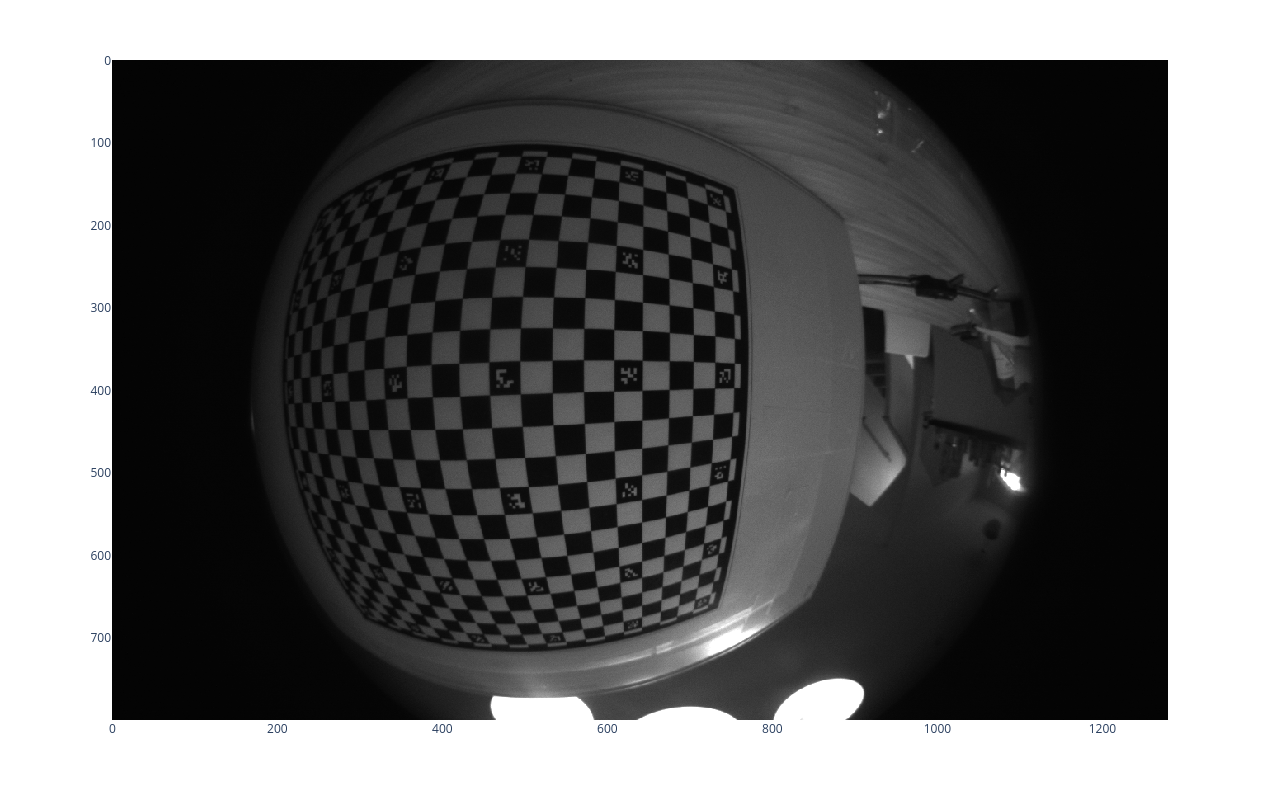
\includegraphics[width=0.10\textwidth]{distorted_image}};
				{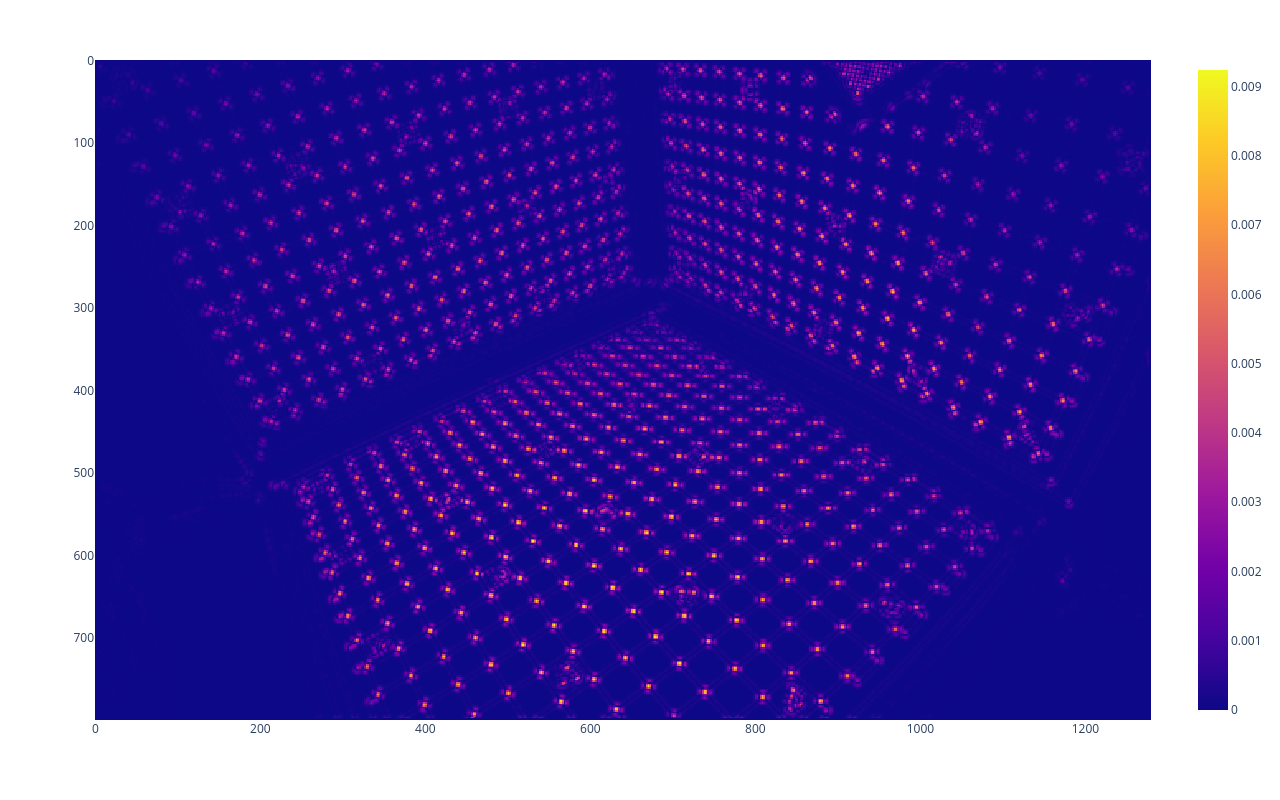
\includegraphics[width=\linewidth]{response_hessian.png}};
				\begin{scope}[x={(image.south east)},y={(image.north west)}]
					\spy[red] on (1.7,1.4) in node [left] at (2.8,3.3);
					% \spy[blue] on (3.5,3.0) in node [right] at (8.1,4.3);
				\end{scope}
			\end{tikzpicture}
			\caption{Hessian response}
		\end{subfigure}
		\begin{subfigure}{0.30\linewidth}
			\begin{tikzpicture}[spy using outlines={circle,yellow,magnification=10,size=3cm, connect spies}]
				\node[anchor=south west,inner sep=0] (image) at (0,0)
				% {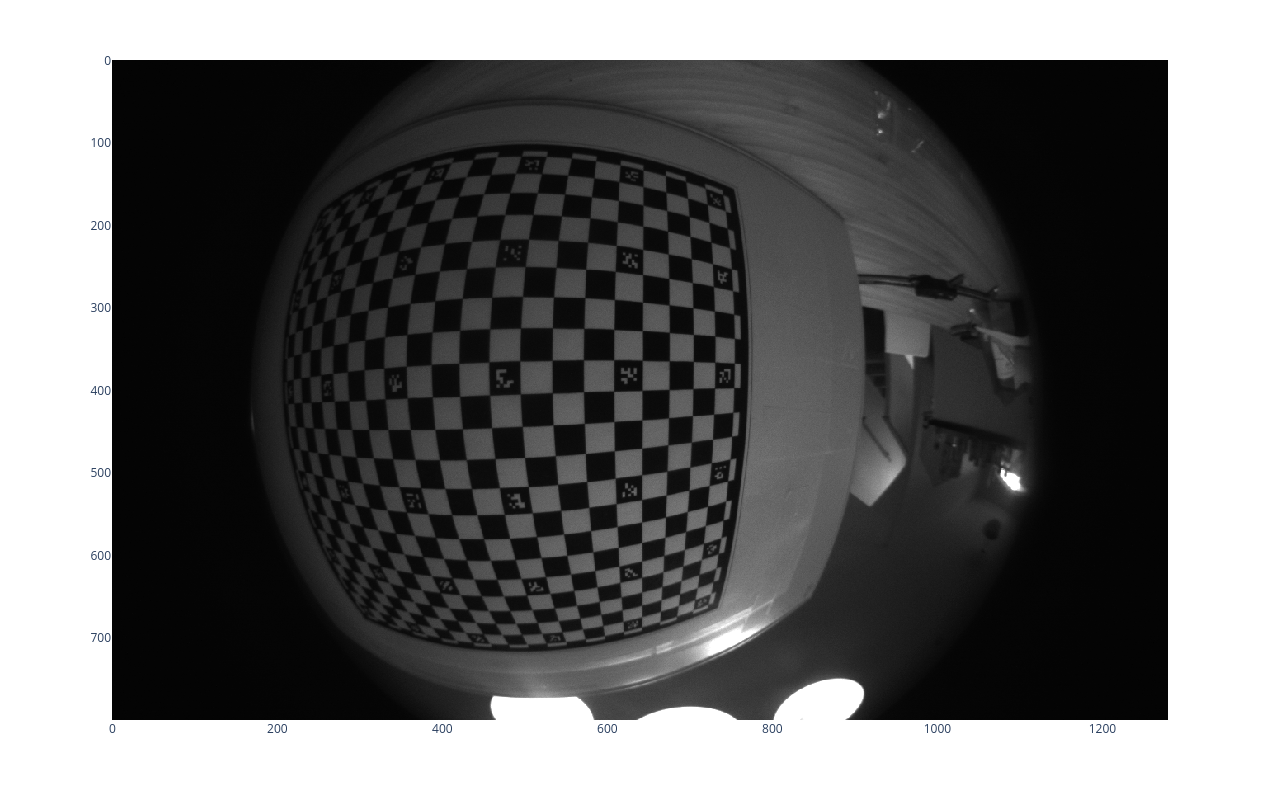
\includegraphics[width=0.6\textwidth]{distorted_image}};
				{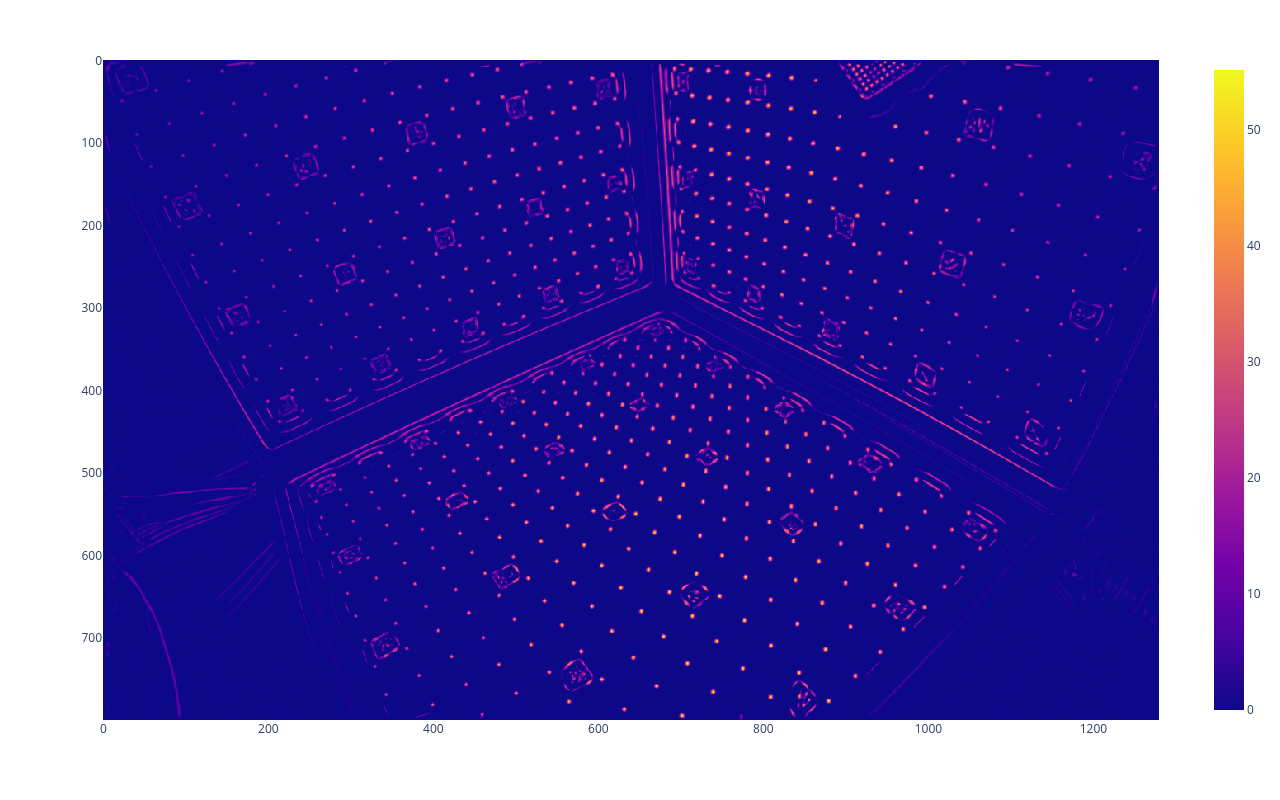
\includegraphics[width=\linewidth]{response_other.png}};
				\begin{scope}[x={(image.south east)},y={(image.north west)}]
					\spy[red] on (1.7,1.4) in node [left] at (2.8,3.3);
					% \spy[blue] on (3.5,3.0) in node [right] at (8.1,4.3);
				\end{scope}
			\end{tikzpicture}
			\caption{\cite{geigerAutomaticCameraRange2012}}
		\end{subfigure}
	\end{figure}

\end{frame}

\begin{frame}
	\frametitle{Evaluation (artificially removed points)}
	We removed 20\% of the points and then tried to recover them.

	\begin{figure}[h]
		\centering
		\begin{subfigure}[h]{\linewidth}
			\resizebox{\linewidth}{!}{
				\begin{tikzpicture}
					\begin{axis}[
							ybar interval,
							ymin=0,
							ylabel={Frequency},
							xlabel={Value},
							height=0.3\linewidth,
							width=\linewidth,
							ticklabel style = {font=\tiny},
							title={Histogram of points before refinement}
						]
						\addplot+ [hist={data min=0,data max=600,bins=10}] table [y index=0]
							% \addplot+ [hist={bins=30}] table [y index=0]
							{data/pruned_number_of_features.txt};
					\end{axis}
				\end{tikzpicture}
			}
		\end{subfigure}
		\hfill
		\begin{subfigure}[h]{\linewidth}
			% \centering
			\resizebox{\linewidth}{!}{
				\begin{tikzpicture}
					\begin{axis}[
							ybar interval,
							ymin=0,
							ylabel={Frequency},
							xlabel={Value},
							height=0.3\linewidth,
							width=\linewidth,
							ticklabel style = {font=\tiny},
							title={Histogram of points after refinement}
						]
						\addplot+ [hist={data min=0,data max=600,bins=10}] table [y index=0]
							% \addplot+ [hist={bins=30}] table [y index=0]
							{data/recovered_pruned_number_of_features.txt};
					\end{axis}
				\end{tikzpicture}
			}
		\end{subfigure}
	\end{figure}

\end{frame}
\begin{frame}
	\frametitle{Evaluation (artificially removed points) 2}

	\begin{figure}
		\begin{tikzpicture}[spy using outlines={circle,yellow,magnification=3,size=4cm, connect spies}]
			\node[anchor=south west,inner sep=0] (image) at (0,0)
			% {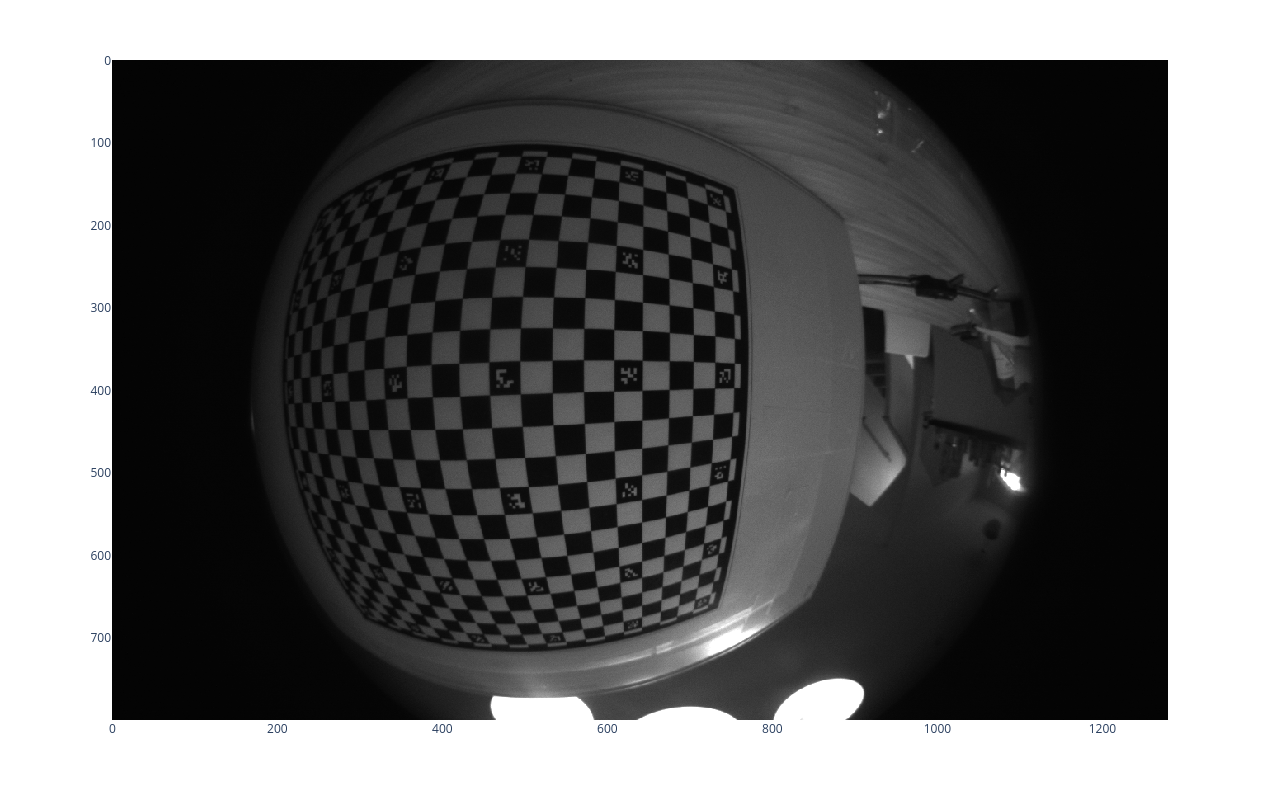
\includegraphics[width=0.6\textwidth]{distorted_image}};
			{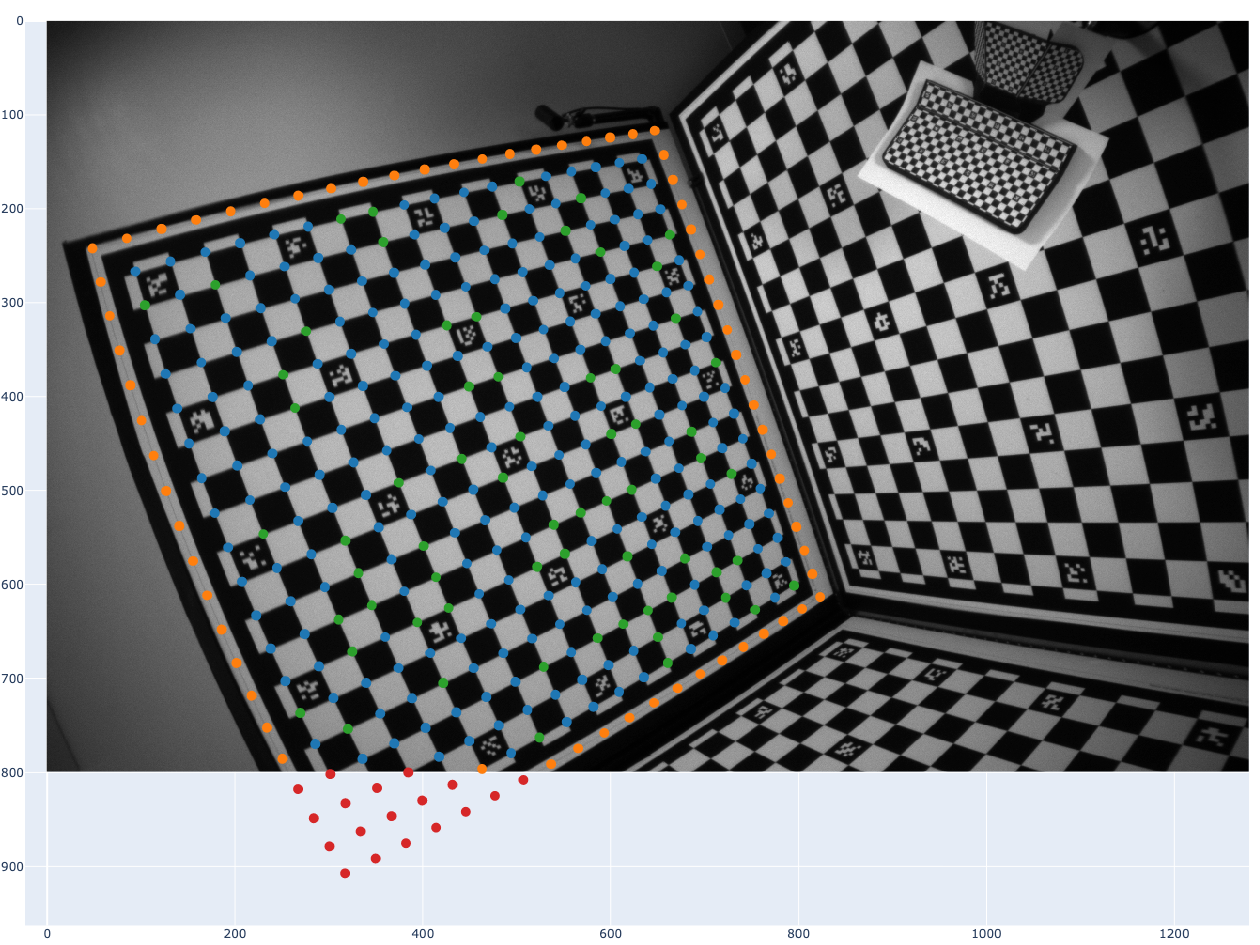
\includegraphics[width=0.7\linewidth]{refined_pruned_corners.png}};
			\begin{scope}[x={(image.south east)},y={(image.north west)}]
				% \spy[red] on (2.5,1.4) in node [left] at (10.1,1.7);
				\spy[blue] on (3.5,3.0) in node [right] at (6.1,3.3);
			\end{scope}
		\end{tikzpicture}
		\caption{Feature recovery on the board with 80\% of the points
			(\textcolor[HTML]{1f77b4}{unchanged}
			\textcolor[HTML]{ff7f0e}{filtered out}
			\textcolor[HTML]{2ca02c}{new corner}
			\textcolor[HTML]{d62728}{out of image})}
	\end{figure}

\end{frame}

\begin{frame}
	\frametitle{Evaluation (artificial occlusion)}

	Occlusions pose complications for feature detection.

	\begin{figure}[h]
		\centering
		\begin{subfigure}[h]{\linewidth}
			\resizebox{\linewidth}{!}{
				\begin{tikzpicture}
					\begin{axis}[
							ybar interval,
							ymin=0,
							ylabel={Frequency},
							xlabel={Value},
							height=0.3\linewidth,
							width=\linewidth,
							ticklabel style = {font=\tiny},
							title={Histogram of points before refinement}
						]
						\addplot+ [hist={data min=0,data max=500,bins=10}] table [y index=0]
							% \addplot+ [hist={bins=30}] table [y index=0]
							{data/occluded_number_of_features.txt};
					\end{axis}
				\end{tikzpicture}
			}
		\end{subfigure}
		\begin{subfigure}[h]{\linewidth}
			% \centering
			\resizebox{\linewidth}{!}{
				\begin{tikzpicture}
					\begin{axis}[
							ybar interval,
							ymin=0,
							ylabel={Frequency},
							xlabel={Value},
							height=0.3\linewidth,
							width=\linewidth,
							ticklabel style = {font=\tiny},
							title={Histogram of points after refinement}
						]
						\addplot+ [hist={data min=0,data max=500,bins=10}] table [y index=0]
							% \addplot+ [hist={bins=30}] table [y index=0]
							{data/recovered_occluded_number_of_features.txt};
					\end{axis}
				\end{tikzpicture}
			}
		\end{subfigure}
	\end{figure}

\end{frame}
\begin{frame}
	\frametitle{Evaluation (artificial occlusion) 2}

	\begin{figure}
		\begin{tikzpicture}[spy using outlines={circle,yellow,magnification=3,size=5cm, connect spies}]
			\node[anchor=south west,inner sep=0] (image) at (0,0)
			% {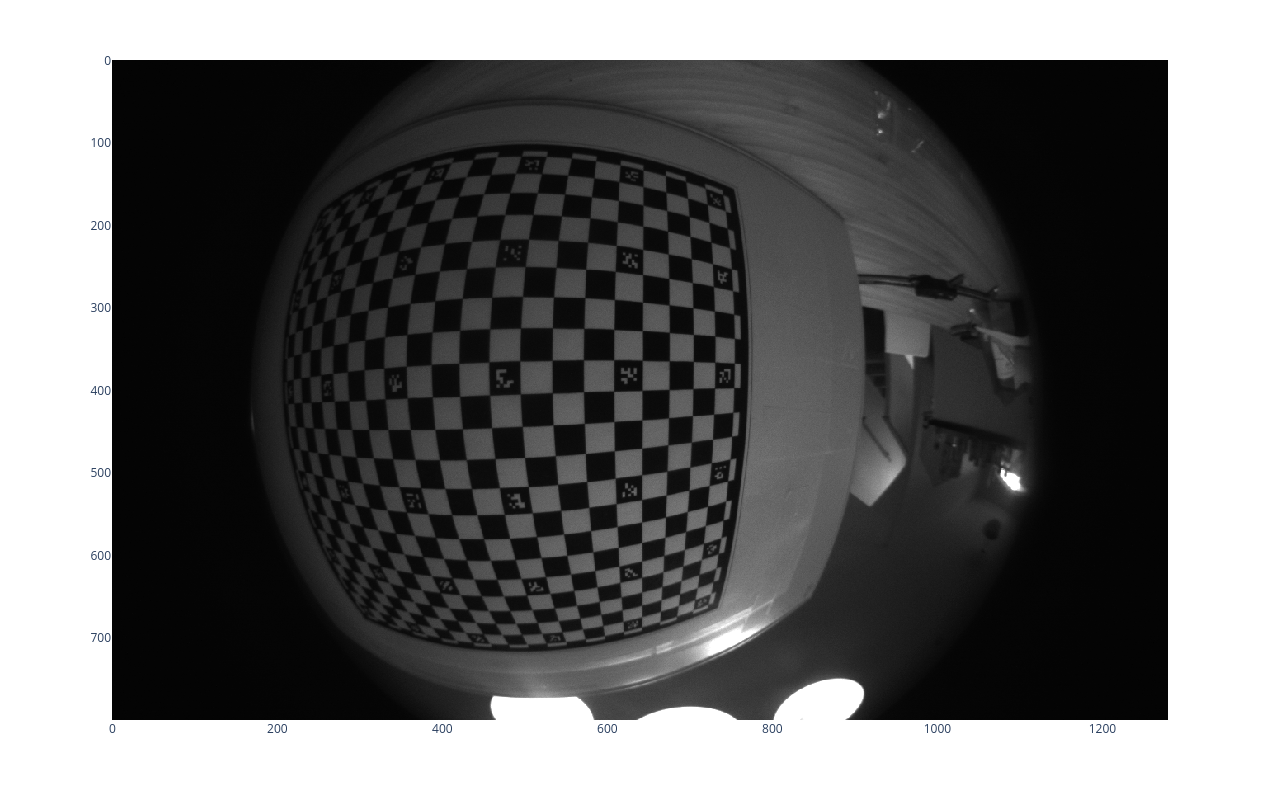
\includegraphics[width=0.6\textwidth]{distorted_image}};
			{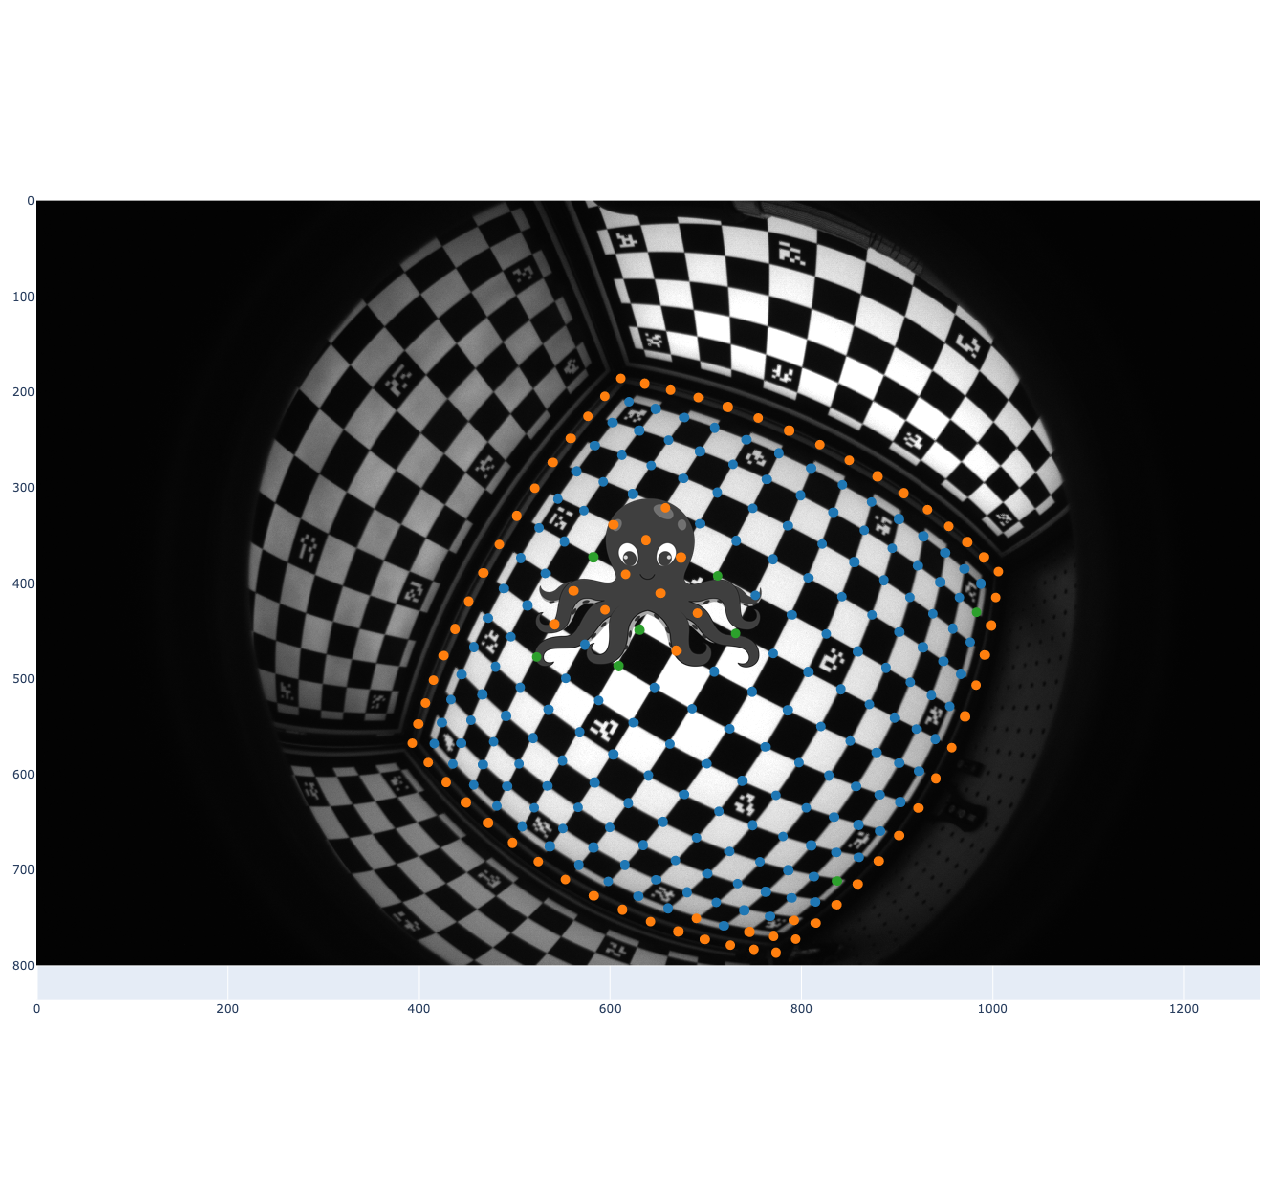
\includegraphics[width=0.7\linewidth]{refined_overlayed_corners.png}};
			\begin{scope}[x={(image.south east)},y={(image.north west)}]
				% \spy[red] on (2.5,1.4) in node [left] at (10.1,1.7);
				\spy[blue] on (3.5,3.0) in node [right] at (6.1,3.3);
			\end{scope}
		\end{tikzpicture}
		\caption{Additional features detection on the board with partial board occlusion
			(\textcolor[HTML]{1f77b4}{unchanged}
			\textcolor[HTML]{ff7f0e}{filtered out}
			\textcolor[HTML]{2ca02c}{new corner}
			\textcolor[HTML]{d62728}{out of image})}
	\end{figure}

\end{frame}

\begin{frame}
	\frametitle{Evaluation (real data)}
	Lastly, we recovered the points that were not detected by the initial feature
	detector.

	\begin{figure}
		\begin{tikzpicture}[spy using outlines={circle,yellow,magnification=4,size=4cm, connect spies}]
			\node[anchor=south west,inner sep=0] (image) at (0,0)
			% {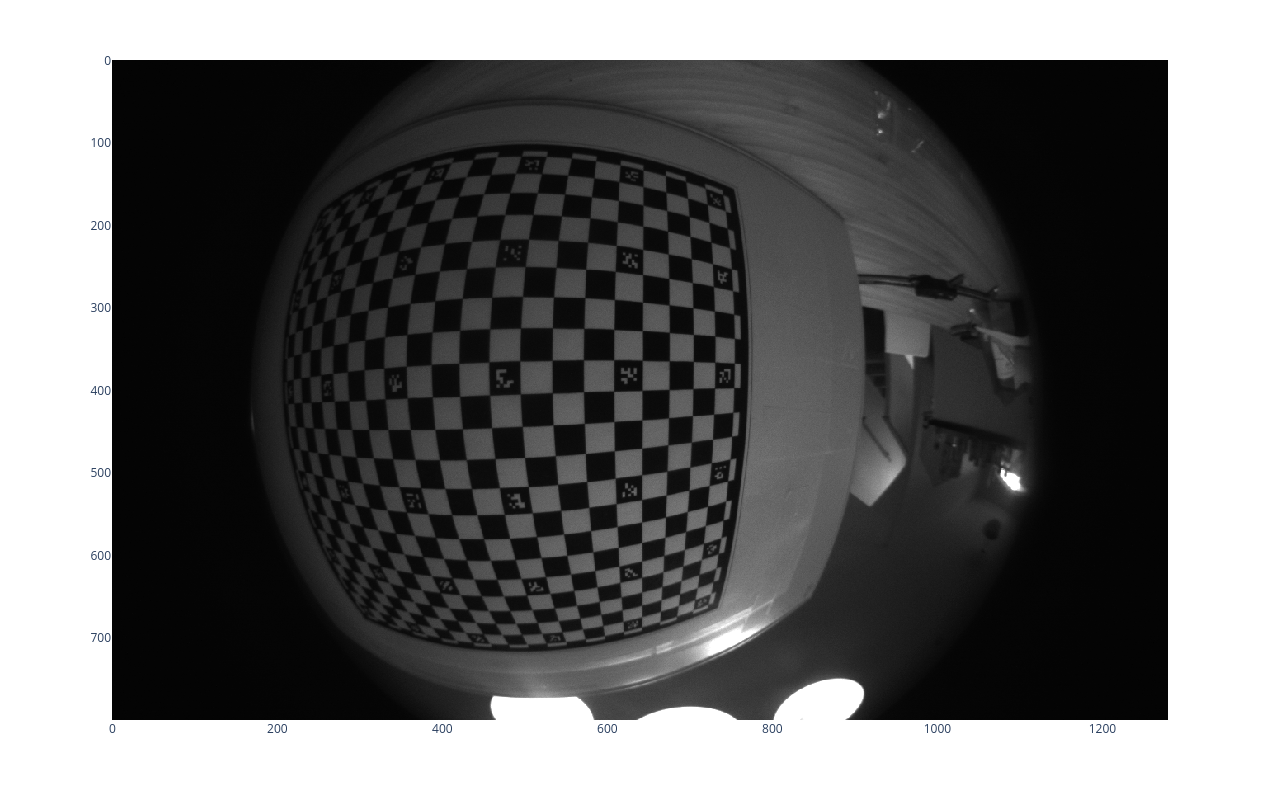
\includegraphics[width=0.6\textwidth]{distorted_image}};
			{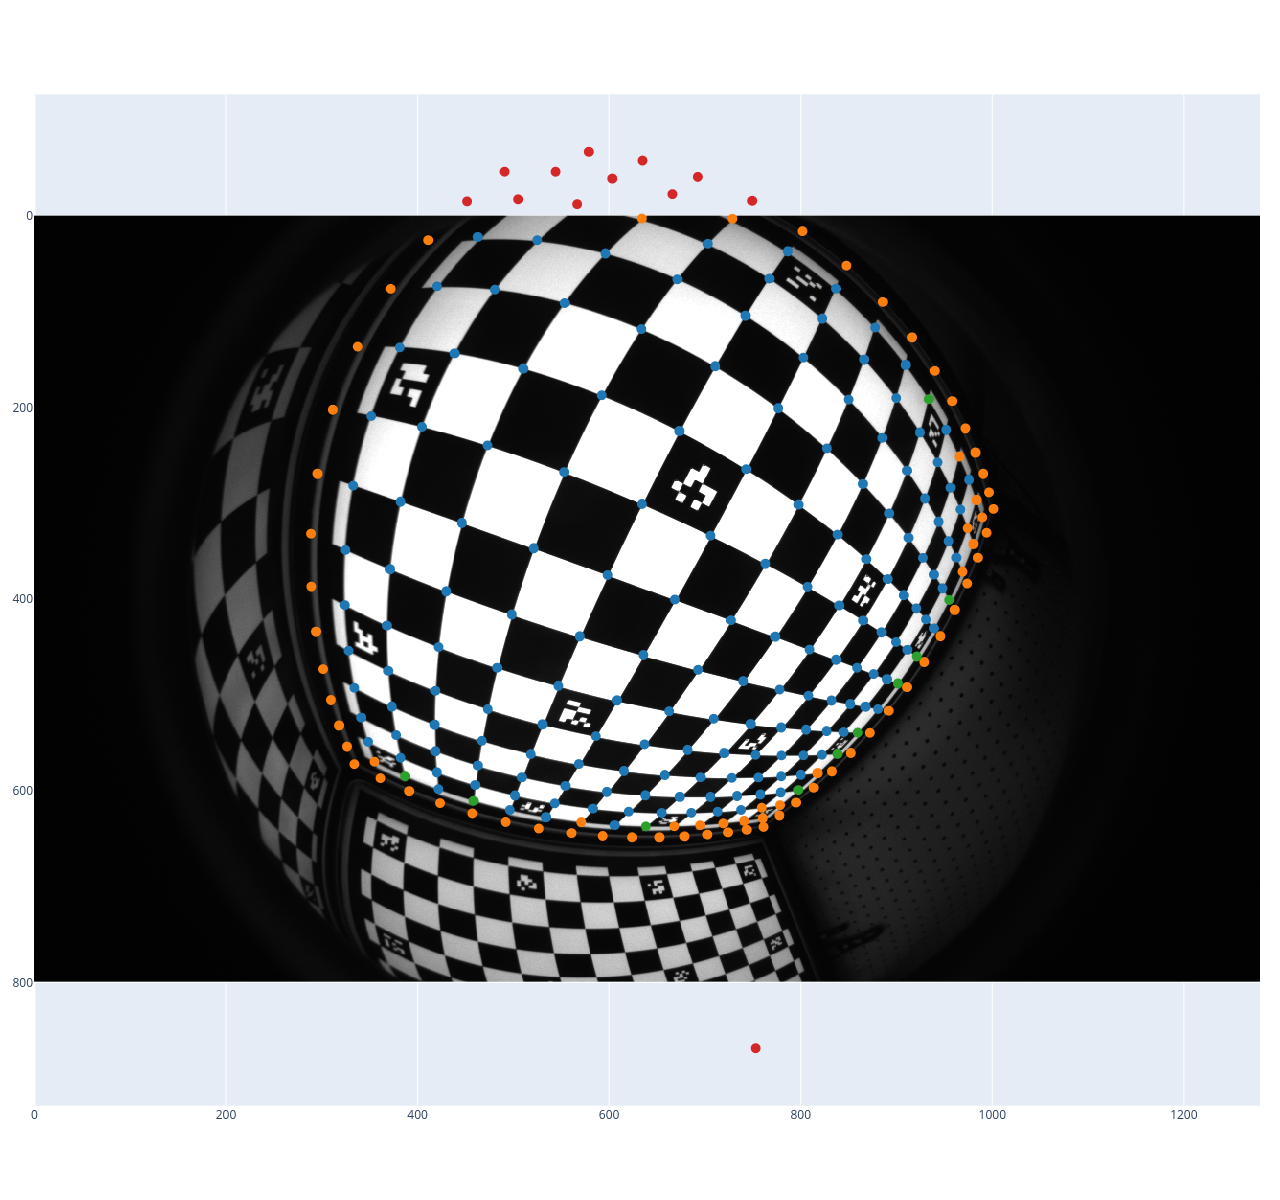
\includegraphics[width=0.6\linewidth]{refined_corners1.png}};
			\begin{scope}[x={(image.south east)},y={(image.north west)}]
				% \spy[red] on (2.5,1.4) in node [left] at (10.1,1.7);
				\spy[blue] on (4.8,2.5) in node [right] at (6.1,3.3);
			\end{scope}
		\end{tikzpicture}
		\caption{Newly detected points
			(\textcolor[HTML]{1f77b4}{unchanged}
			\textcolor[HTML]{ff7f0e}{filtered out}
			\textcolor[HTML]{2ca02c}{new corner}
			\textcolor[HTML]{d62728}{out of image})}
	\end{figure}

\end{frame}

\begin{frame}
	\frametitle{Evaluation (real data) 2}

	\begin{figure}
		\begin{tikzpicture}[spy using outlines={circle,yellow,magnification=4,size=5cm, connect spies}]
			\node[anchor=south west,inner sep=0] (image) at (0,0)
			% {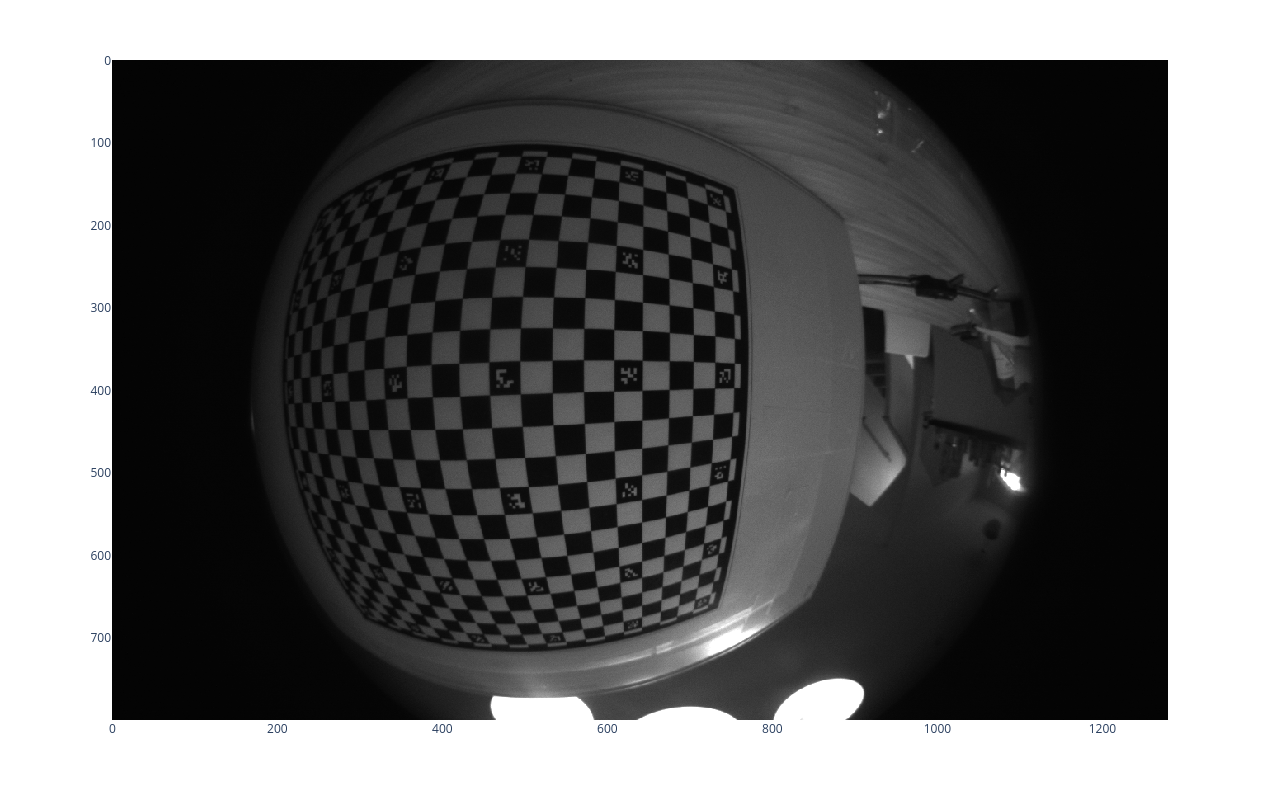
\includegraphics[width=0.6\textwidth]{distorted_image}};
			{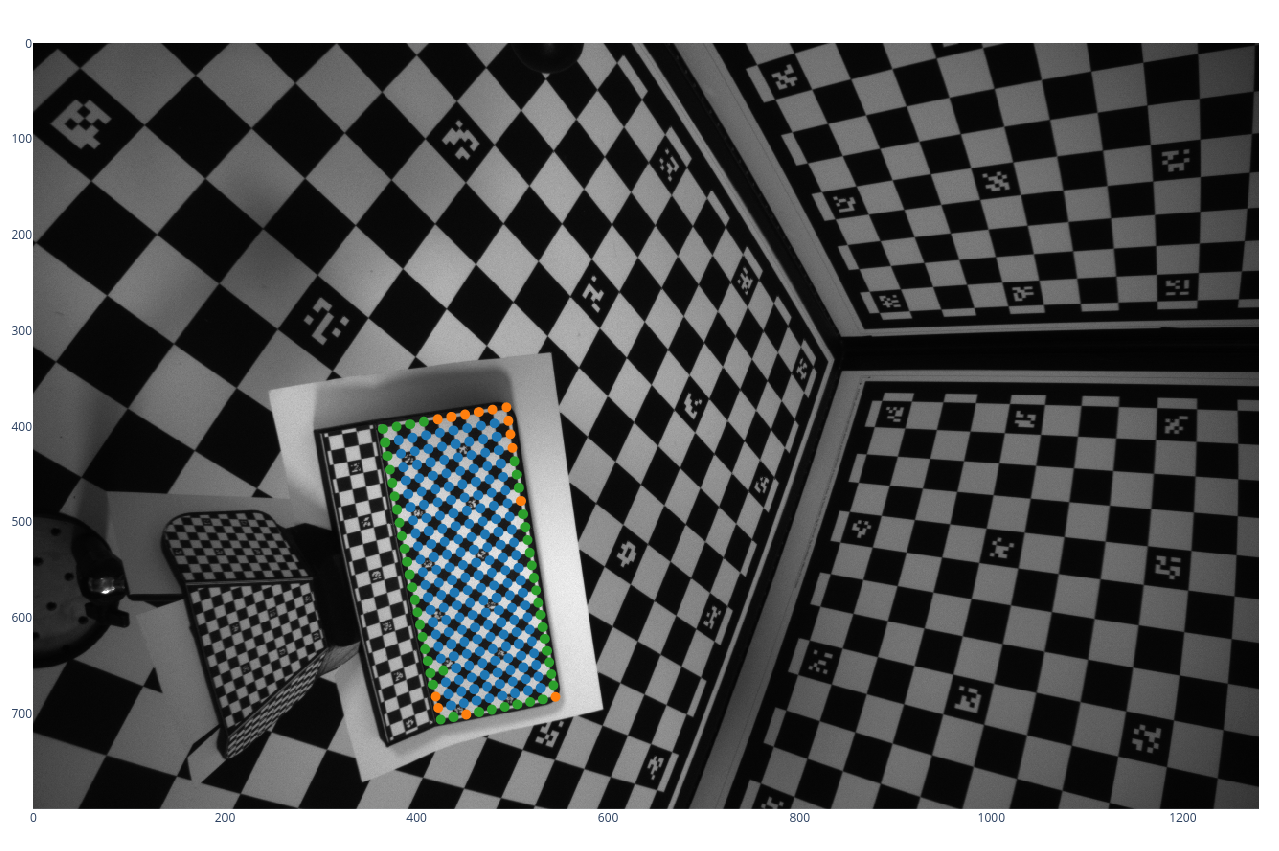
\includegraphics[width=0.75\linewidth]{refined_corners2.png}};
			\begin{scope}[x={(image.south east)},y={(image.north west)}]
				% \spy[red] on (2.5,1.4) in node [left] at (10.1,1.7);
				\spy[blue] on (3.0,2.4) in node [right] at (6.1,3.3);
			\end{scope}
		\end{tikzpicture}
		\caption{Newly detected points
			(\textcolor[HTML]{1f77b4}{unchanged}
			\textcolor[HTML]{ff7f0e}{filtered out}
			\textcolor[HTML]{2ca02c}{new corner}
			\textcolor[HTML]{d62728}{out of image})}
	\end{figure}
\end{frame}

\begin{frame}
	\frametitle{Evaluation (real data, false positives)}

	\begin{figure}
		\begin{tikzpicture}[spy using outlines={circle,yellow,magnification=4,size=5cm, connect spies}]
			\node[anchor=south west,inner sep=0] (image) at (0,0)
			% {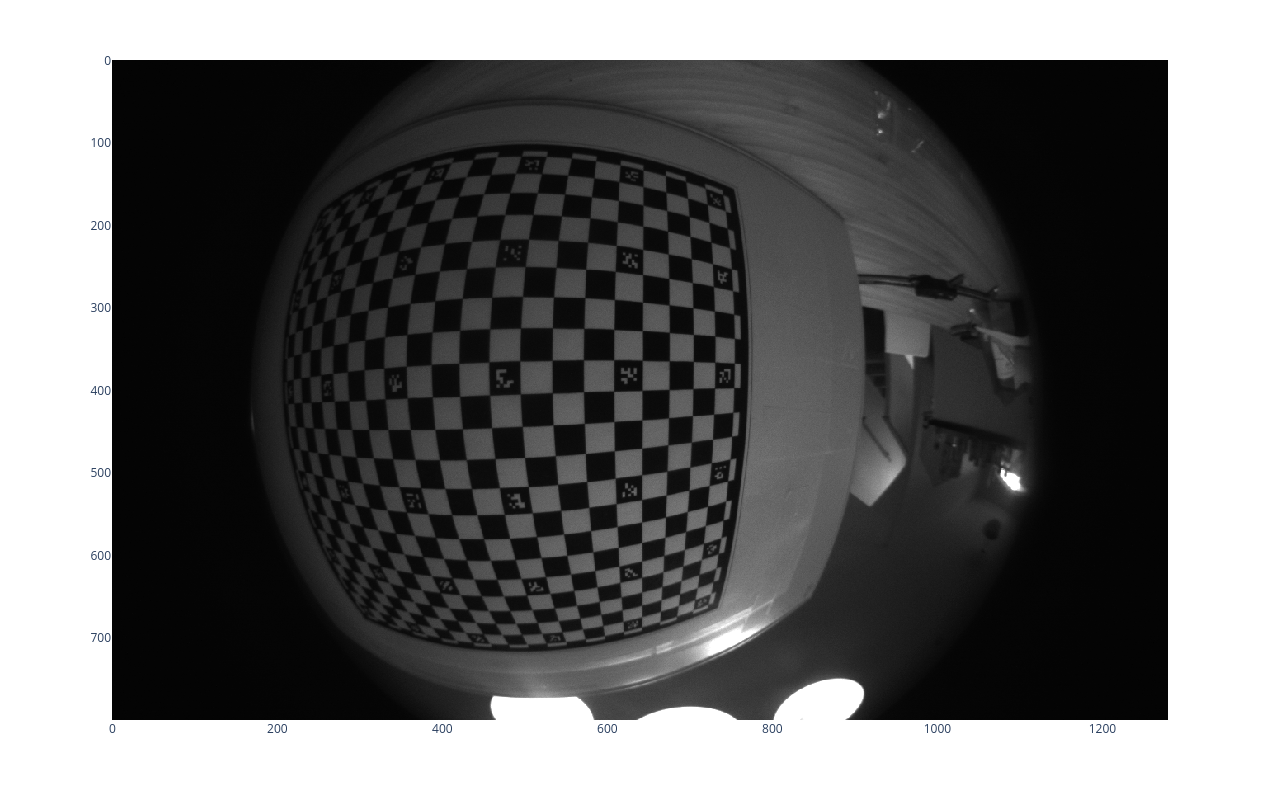
\includegraphics[width=0.6\textwidth]{distorted_image}};
			{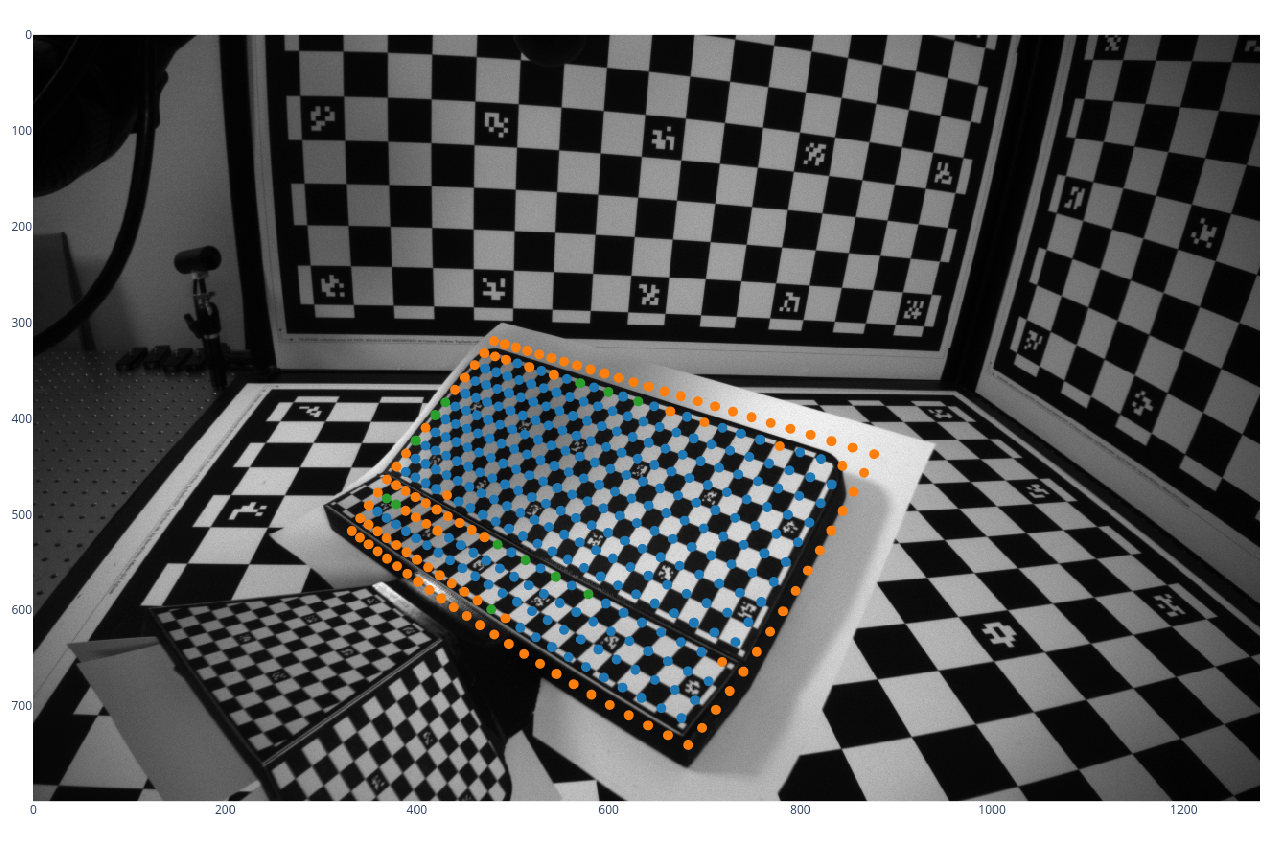
\includegraphics[width=0.7\linewidth]{refined_corners_bad_bad.png}};
			\begin{scope}[x={(image.south east)},y={(image.north west)}]
				% \spy[red] on (2.5,1.4) in node [left] at (10.1,1.7);
				\spy[blue] on (2.6,2.0) in node [right] at (6.1,3.3);
			\end{scope}
		\end{tikzpicture}
		\caption{Example of false positives
			(\textcolor[HTML]{1f77b4}{unchanged}
			\textcolor[HTML]{ff7f0e}{filtered out}
			\textcolor[HTML]{2ca02c}{new corner}
			\textcolor[HTML]{d62728}{out of image})}
	\end{figure}

\end{frame}

\begin{frame}
	\frametitle{Evaluation (real data)}

	\begin{figure}[h!]
		\begin{tikzpicture}
			\begin{axis}			[
					ymode=log,
					ybar interval,
					ylabel={Frequency},
					xlabel={Value},
					height=0.3\linewidth,
					width=\linewidth,
					ticklabel style = {font=\tiny},
					% title={Initial calibration}
				]
				\addplot+ [hist={data min=0,data max=50,bins=20}] table [y index=0]
					% \addplot+ [hist={bins=30}] table [y index=0]
					{data/number_of_refined_points.txt};
			\end{axis}
		\end{tikzpicture}
		\caption{Histogram of the newly recovered features}
		\label{fig:recovered_points_histogram}
	\end{figure}

\end{frame}

\begin{frame}
	\frametitle{Comparison}
	\begingroup
	\scriptsize

	\setlength\tabcolsep{1.5pt} % default value: 6pt
	\begin{table}
		\begin{tabularx}{\textwidth}{@{} L *{6}{c} @{}}
			\toprule
			\multicolumn{1}{c}{\multirow{2}{*}{\centering\textbf{Supports}}}           &
			\multicolumn{6}{c@{}}{\textbf{Name}}                                                                  \\
			\cmidrule(l){2-7}                                                          &
			\textbf{OpenCV\footcite{dudaAccurateDetectionLocalization2018}}            &
			\textbf{TartanKalib\footcite{duisterhofTartanCalibIterativeWideAngle2022}} &
			\textbf{Kalibr\footcite{mayeSelfsupervisedCalibrationRobotic2013}}         &
			\textbf{OCamCalib\footcite{scaramuzzaToolboxEasilyCalibrating2006}}        &
			\textbf{LIBCBDETECT\footcite{geigerAutomaticCameraRange2012}}              &
			{\normalsize \textbf{Ours}}                                                                           \\
			\midrule
			Unknown board shape                                                        & \xmark & \cmark & \cmark
			                                                                           & \cmark & \cmark & \cmark \\
			\hline
			Occlusion                                                                  & \xmark & \cmark & \cmark
			                                                                           & \cmark & \cmark & \cmark \\
			\hline
			Model-based extra features detection                                       & \xmark & \cmark & \xmark
			                                                                           & \xmark & \xmark & \cmark \\
			\hline
			Geometry-based extra features detection                                    & \xmark & \xmark & \xmark
			                                                                           & \xmark & \xmark & \cmark \\
			\bottomrule
		\end{tabularx}
		\caption{Comparison of feature detectors}
	\end{table}
	\endgroup
\end{frame}

\section{Conclusions}\label{sec:conclusions}

\begin{frame}
	\frametitle{Answers to the research questions}

	\begin{itemize}
		\item \textbf{How to find additional features on the calibration board which were not
			      detected by the feature detector?}\\

		      This thesis proposes a model-based approach to improve the detection of
		      calibration board fiducials from calibration imagery taken by wide-angle or
		      fisheye lenses.
		\item \textbf{How to filter out falsely detected features?}\\

		      We proposed a classifier that filters false positives, and
		      shown that it works well on real data.
		\item \textbf{Is there a need for finding additional features on the calibration
			      board? Are all of the points detected?}\\

		      We demonstrated that the proposed method successfully detected
		      additional features on the real data.
	\end{itemize}
\end{frame}

\begin{frame}
	\frametitle{Reviewers' comments 1}
	\textbf{No comparison was made to classical camera calibration results}

	The main contribution is the feature detection step.

	The algorithm estimates camera parameters, but we don't claim that they are
	better than state-of-the-art. The user can use those, or pass the refined
	features into any camera calibration toolchain.
	% The user can use the
	% obtained camera parameters, however, we do not claim that they will always beat the
	% SOTA. Alternatively, the user should pass the refined features to any camera
	% calibration toolchain.
\end{frame}

\begin{frame}
	\frametitle{Reviewers' comments 2}
	\textbf{The literature review
		does not include a review of methods that solve the feature detection step in
		a different way}

	A review of feature detection methods is presented in the paper.

	The specific subtask of model-based missed
	feature detection is not big enough to have a separate review. However, we
	included TartanKalib\footcite{duisterhofTartanCalibIterativeWideAngle2022}.
\end{frame}

\begin{frame}
	\frametitle{Reviewers' comments 3}
	\textbf{There is no general block diagram of the algorithm}

	\begin{figure}
		\begin{tikzpicture}[
				block/.style={rectangle, draw, align=center, minimum width=2cm, minimum
						height=1cm, font=\footnotesize},
				line/.style={draw, -latex}
			]
			\node [block] (block1) {Feature\\ detection};
			\node [block, right=of block1, minimum width=8cm, minimum height=3cm] (block2) {};
			\node [block, at={(block2.center)}, xshift=-2.0cm] (block3) {Initialize camera\\ parameters (\(R\), \(\mathbf{t}\), \(\boldsymbol{\lambda}\))\\ using the solver};
			\node [block, at={(block2.center)}, xshift=2.0cm] (block4) {Refine camera\\ parameters and\\ estimate \(K\)\\ by optimization};
			\node [block, below=of block4] (block5) {Impute the gaps in\\ the board, and\\ extend it};
			\node [block, left=of block5] (block6) {Get positions of\\ new points on\\ the image};
			\node [block, left=of block6] (block7) {Filter out\\ false positives};

			\node [above of=block2, node distance=1.8cm] {Camera calibration};

			\path [line] (block1) -- (block3);
			\path [line] (block3) -- (block4);
			% \path [line] (block2) -| (block3);
			% \path [line] (block2) -| (block4);
			% \path [line] (block3) -- (block5);
			\path [line] (block4) -- (block5);
			\path [line] (block5) -- (block6);
			\path [line] (block6) -- (block7);
		\end{tikzpicture}
	\end{figure}
\end{frame}

\begin{frame}
	\frametitle{Reviewers' comments 4}
	\textbf{It is not sufficiently described what results are obtained on
		test sets}

	The datasets we used did not contain the ground truth camera calibration.
	Also, the algorithm does not include the learning step, hence there is no
	reason to use the test set.
	% Also, we used three datasets with different setup.
\end{frame}

\begin{frame}
	\frametitle{Reviewers' comments 4}
	\textbf{The questions "How to filter incorrectly defined grid points" and "Is there a
		need to search for additional grid points" posed in the work are insufficiently disclosed}

	Addressed in section Conclusions.
\end{frame}

\begin{frame}
	\frametitle{Reviewers' comments 5}
	\textbf{A comparison of the results with other feature detection methods has not been made}

	We have added a feature-wise comparison to the state-of-the-art methods, and
	numerical comparison to the
	LIBCBDETECT\footcite{geigerAutomaticCameraRange2012} method.

	The TartanKalib\footcite{duisterhofTartanCalibIterativeWideAngle2022} method
	currently supports only AprilGrid boards.
\end{frame}

\begin{frame}[standout]
	Q\&A

\end{frame}

\appendix

\begin{frame}
	\frametitle{Extrinsic parameters}
	The extrinsic parameters represent a rigid transformation from a 3-D world
	coordinate system to the 3-D camera’s coordinate system.

	\begin{exampleblock}{Definition}
		\begin{equation*}
			\widehat{\mathbf{x}} =
			R \begin{pmatrix}
				x, y, z
			\end{pmatrix}^{T} + \mathbf{t} =
			\begin{bmatrix}
				R              & \mathbf{t} \\
				\mathbf{0}^{T} & 1
			\end{bmatrix} \begin{pmatrix}
				x, y, z, 1
			\end{pmatrix}^{T},
		\end{equation*}
		where
		\(\begin{pmatrix}
			x, y, z
		\end{pmatrix}^{T}\) is a 3D scene point,
		% \(R \begin{pmatrix}
		% 	x, y, z
		% \end{pmatrix}^{T} + \mathbf{t}\), where
		\(R\) is a \(3 \times 3\) rotation matrix
		and \(\mathbf{t}\) is
		a \(3 \times 1\) translation vector.
	\end{exampleblock}
\end{frame}

\begin{frame}
	\frametitle{Extrinsic parameters}

	When working with the coplanar scene points, we can simplify the projection
	by assuming that the scene plane is located at \(Z = 0\). In this case, the
	projection of the point becomes:
	\begin{exampleblock}{Definition for coplanar points}
		\begin{equation*}
			\alpha \begin{pmatrix}
				u \\ v \\ 1
			\end{pmatrix} = \begin{bmatrix}
				\mathbf{r_1} & \mathbf{r_2} & \mathbf{r_3} & \mathbf{t}
			\end{bmatrix} \begin{pmatrix}
				x \\ y \\ 0 \\ 1
				% \end{pmatrix} = \begin{bmatrix}
				%   \mathbf{p_1} & \mathbf{p_2} & \mathbf{p_4}
				% \end{bmatrix} \begin{pmatrix}
				%   x \\ y \\ 1
				% \end{pmatrix}.
			\end{pmatrix} = \underbrace{\begin{bmatrix}
					\mathbf{r_1} & \mathbf{r_2} & \mathbf{t}
				\end{bmatrix}}_{H} \begin{pmatrix}
				x \\ y \\ 1
			\end{pmatrix}.
		\end{equation*}
	\end{exampleblock}
\end{frame}

\begin{frame}
	\frametitle{Distortion model}
	The distortion of the image is caused by the lens not being perfectly planar.
	We used the division distortion model
	\cite{fitzgibbonSimultaneousLinearEstimation2001} which maps a
	point from a retinal plane to the
	ray direction in the camera coordinate system.
	\begin{exampleblock}{Definition}
		\begin{equation*}
			g(\mathbf{u}) = \begin{pmatrix}
				u, v, \psi(r(\mathbf{u}))
			\end{pmatrix}^{T},
			\psi(r) = 1 + \sum_{n = 1}^{N} \lambda_n r^{2n},
		\end{equation*}
		where
		\(\mathbf{u} = \begin{pmatrix}
			u, v, 1
		\end{pmatrix}^{T}\) is a point in the retinal plane
		, \(r(\mathbf{u}) = \sqrt{u^2 + v^2}\) is the radial distance from the
		principal point and \(\lambda_n\) are the distortion coefficients.
	\end{exampleblock}
\end{frame}

\begin{frame}
	\frametitle{Intrinsic parameters}
	Represent a projective transformation from the 3-D camera’s coordinates into
	the 2-D image coordinates.

	\begin{exampleblock}{Definition}
		\begin{equation*}
			K = \begin{bmatrix}
				\alpha_x & \alpha_x \cot \theta & c_x \\
				0        & \alpha_y             & c_y \\
				0        & 0                    & 1
			\end{bmatrix} \begin{bmatrix}
				f & 0 & 0 \\
				0 & f & 0 \\
				0 & 0 & 1
			\end{bmatrix} = \begin{bmatrix}
				f_x & k   & c_x \\
				0   & f_y & c_y \\
				0   & 0   & 1
			\end{bmatrix}.
		\end{equation*}
		For a typical camera, \(\theta = \sfrac{\pi}{2}\) and \(\alpha_x = \alpha_y\)
		\cite{hartleyMultipleViewGeometry2004}:
		\begin{equation*}
			K = \begin{bmatrix}
				f & 0 & c_x \\
				0 & f & c_y \\
				0 & 0 & 1
			\end{bmatrix}.
		\end{equation*}
	\end{exampleblock}

\end{frame}

\end{document}
